\documentclass[12pt,halfparskip]{scrartcl}

\newcommand{\dokumenttitel}{Design}
\usepackage{../bodesuri}
\usepackage{float}

\begin{document}

\title{\dokumenttitel}
\titlehead{
	\centering
	
\includegraphics[width=0.5 \textwidth, clip, trim = 0 7cm 0 0]{design/externes_design/bodesuri_plakat}
	\vspace{2cm}
}
\author{Danilo~Couto, Philippe~Eberli, \\ Pascal~Hobus, Reto~Schüttel, Robin~Stocker}
\maketitle
\newpage

\pagenumbering{roman}

\tableofcontents
\thispagestyle{plain}
\newpage

\pagenumbering{arabic}

\markright{Bodesuri -- \dokumenttitel}


\section{Architekturübersicht}

Bodesuri ist über mehrere Rechner verteilt. Es gibt vier Clients und einen Server pro Spiel. Der Client und der Server sind getrennte Programme, welche aber eine gemeinsame Codebasis haben.

Zwischen Client und Server werden Nachrichten verschiedener Typen zur Synchronisation ausgetauscht. Ein Beispiel anhand der Züge: Der Server sendet dem Spieler, der am Zug ist, eine Zugaufforderung. Auf die antwortet der Spieler mit einem Zug, welcher den Spieler, die gezogene Karte und die Bewegung der Figuren enthält. Der Server verteilt dann diese Informationen als Zuginformation an alle Spieler, wie man in Abbildung~\vref{fig:client_server} sehen kann.

\begin{figure}[h]
	\centering
	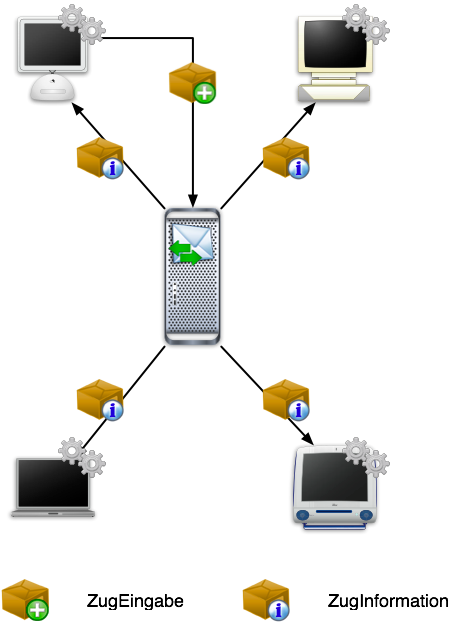
\includegraphics[width=0.6 \textwidth]{client_server}
	\caption{Kommunikation zwischen Client \& Server}
	\label{fig:client_server}
\end{figure}

Die Validierung der gespielten Züge geschieht sowohl auf dem Client als auch auf dem Server. Der Server ist ausserdem noch zuständig für die Koordination des Spielablaufs und für die Kommunikation zwischen den Spielern.

\clearpage
\section{Logische Sicht}

Die logische Sicht zeigt die Aufteilung des Designs in Schichten und Packages.

\subsection{Schichtenarchitektur}

Für die logische Strukturierung des Projektes wird eine vierschichtige Architektur verwendet, wie in Abbildung~\vref{fig:architektur_schichten} dargestellt. Dabei setzt jede Schicht direkt auf den Diensten der darunterliegenden Schichten auf. Schichten können transparent sein. Dadurch ergeben sich wenige Indirektionen und eine einfache Nutzung der Dienste einer Schicht. Wo möglich und sinnvoll, werden Schnittstellen zwischen Schichten durch eine Fassade gebündelt, um die Kopplung zwischen den Schichten zu verringern. Dadurch lassen sich die Schnittstellen für die Schichten auch klarer definieren und sind einfacher zu nutzen. Im UI wird das MVC-Konzept verwendet, da eine komplexe Darstellungslogik durch das Spiel gegeben ist.
\begin{figure}
	\centering
	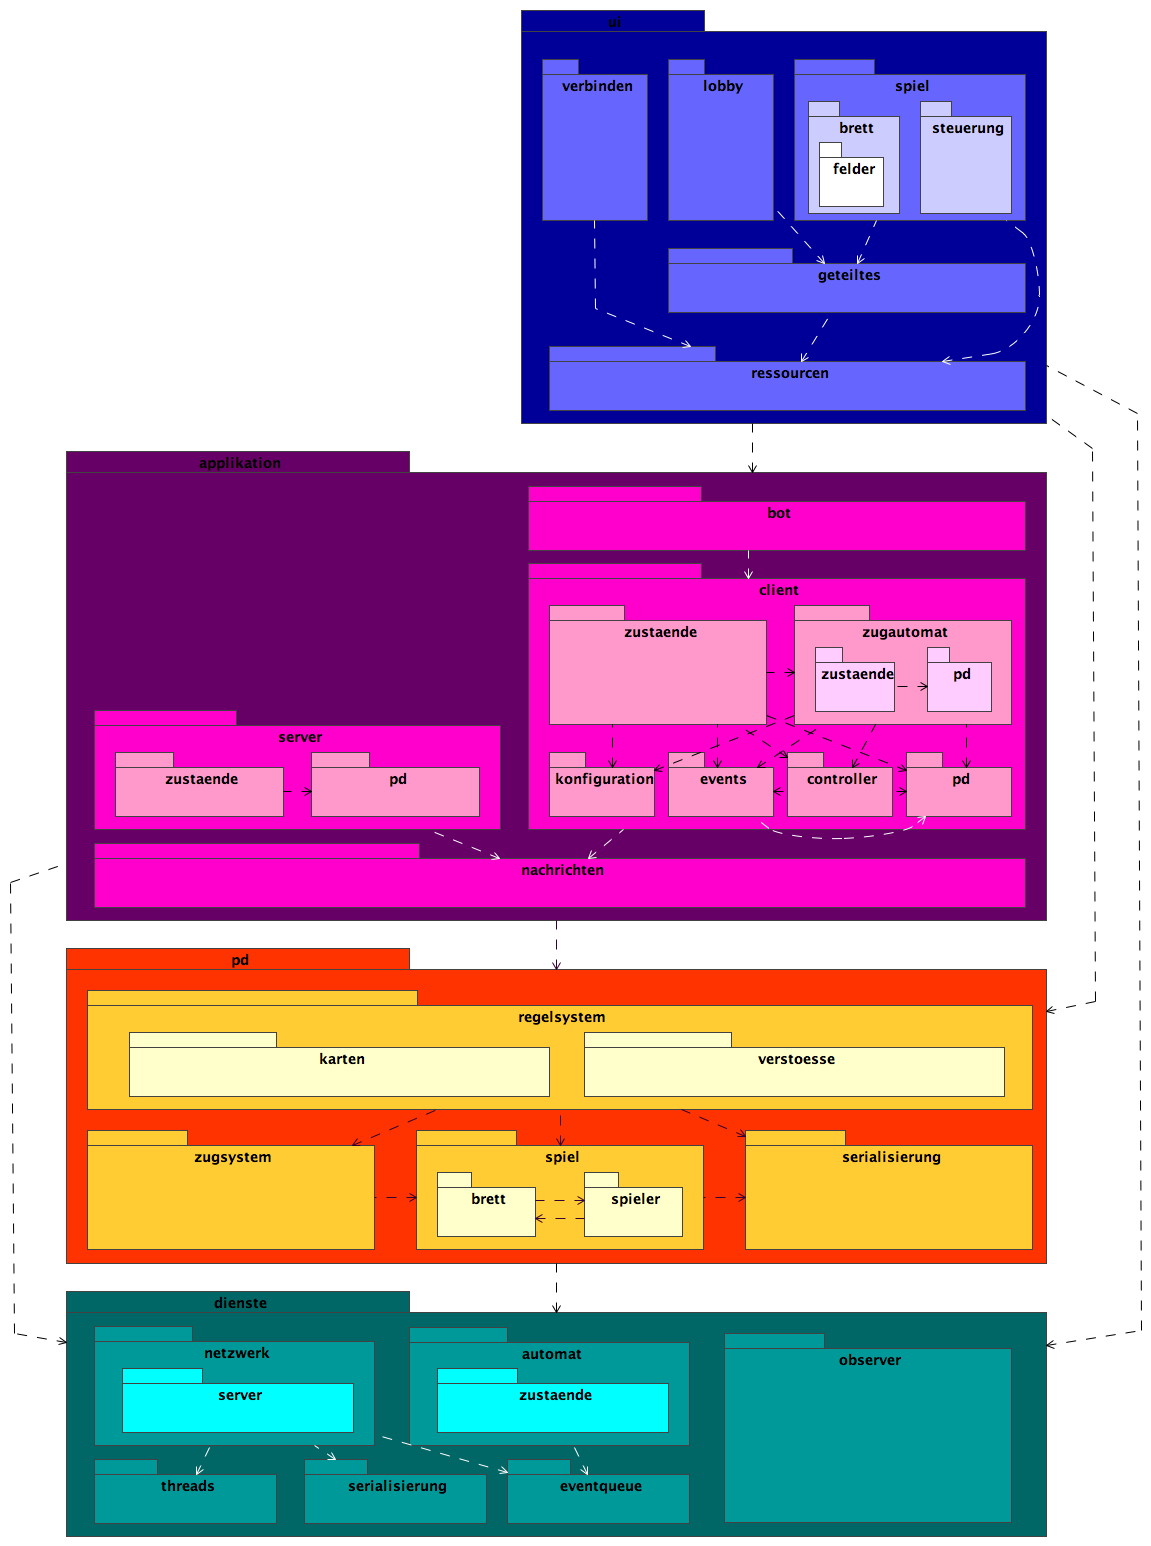
\includegraphics[width=\textwidth]{architektur_schichten}
	\caption{Schichtenarchitektur}
	\label{fig:architektur_schichten}
\end{figure}

\clearpage

\subsection{Package pd}

In der Problem-Domain-Schicht wird die gesamte Spiellogik gekapselt. Sie wird direkt von der darüberliegenden Applikationsschicht verwendet.

\paragraph{Schnittstellen}
\begin{itemize}
	\item Der Einstiegspunkt ist die Klasse ProblemDomain, welche für das Erstellen eines Spiels (pd.spiel), eines KartenGebers (pd.regelsystem.karten) und eines Codierers (dienste.serialisierung).
\end{itemize}

\begin{figure}[H]
	\centering
	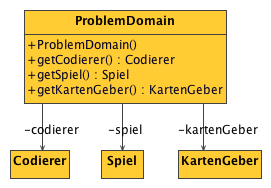
\includegraphics[width=0.6 \textwidth]{kd_pd}
	\caption{Klassendiagramm ProblemDomain}
	\label{fig:kd_pd}
\end{figure}

\clearpage
\subsection{Package pd.spiel}

Das Package pd.spiel beinhaltet die Spiel-Klasse und die folgenden  Unterpackages:

\begin{itemize}
	\item \textbf{pd.spiel.brett} Brett und alle Feldtypen.
	\item \textbf{pd.spiel.spieler} Spieler, SpielerFarbe, Figuren und Partnerschaft
\end{itemize}

\paragraph{Schnittstellen}
\begin{itemize}
	\item Ein Spiel beinhaltet ein Brett und die Spieler. Es sollte nie direkt erstellt werden sondern nur von der Klasse ProblemDomain (pd).
\end{itemize}

\begin{figure}[H]
	\centering
	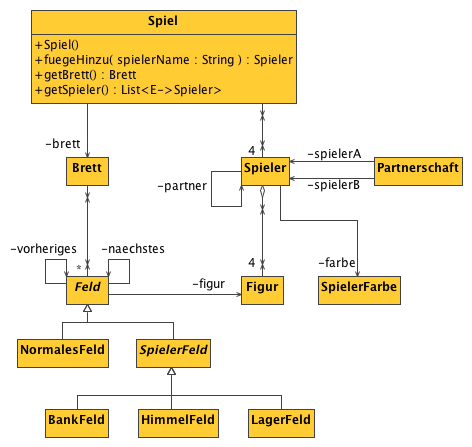
\includegraphics[width=0.9 \textwidth]{kd_pd_spiel}
	\caption{Klassendiagramm Spiel in PD}
	\label{fig:kd_pd_spiel}
\end{figure}

\clearpage
\subsection{Package pd.regelsystem}

Das Regelsystem nimmt die Aufgaben der Problem-Domain-Schicht wahr, indem sie die Validierung der Züge sicherstellt und die daraus resultierenden Aktionen in der Problem-Domain berechnet (Figur von Feld X auf Feld Y verschieben). Beinhaltet zwei Subpackages:

\begin{itemize}
	\item \textbf{pd.regelsystem.karten} Karten, KartenFarbe, Deck und KartenGeber
	\item \textbf{pd.regelsystem.verstoesse} RegelVerstoss und abgeleitete Klassen
\end{itemize}

\paragraph{Schnittstellen}
\begin{itemize}
	\item Die Zugeingabe fasst die Informationen zusammen, die für einen Zug benötigt werden. Sie wird von einer Regel validiert, was einen ausführbaren Zug (in pd.zugsystem) als Ergebnis hat.
\end{itemize}

\begin{figure}[H]
	\centering
	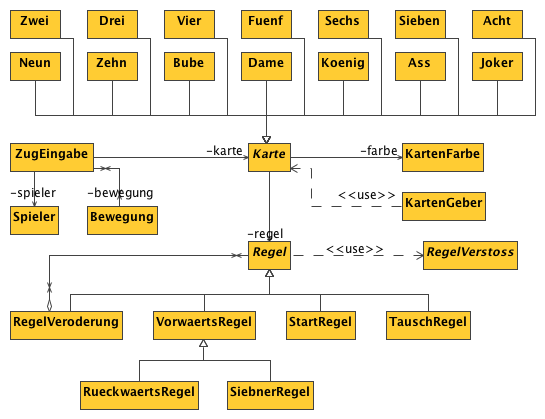
\includegraphics[width=\textwidth]{kd_pd_regelsystem}
	\caption{Klassendiagramm Regelsystem}
	\label{fig:kd_pd_regelsystem}
\end{figure}

\clearpage
\subsection{Package pd.zugsystem}

Das Zugsystem stellt hauptsächlich Klassen bereit, die vom Regelsystem verwendet werden. So wird zum Beispiel vom Regelsystem aus einer Zugeingabe ein Zug mit Aktionen erstellt. Bewegung und Weg sind Hilfsklassen für die Validierung.

\begin{figure}[H]
	\centering
	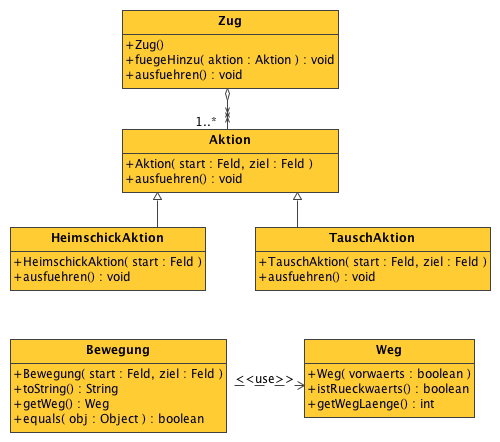
\includegraphics[width=0.8 \textwidth]{kd_pd_zugsystem}
	\caption{Klassendiagramm Zugsystem}
	\label{fig:kd_pd_zugsystem}
\end{figure}

\clearpage
\subsection{Package pd.serialisierung}

Implementiert die abstrakten Klassen von dienste.serialisierung, um die Serialisierung von Klassen der Problem-Domain zu ermöglichen.

\paragraph{Schnittstellen}
\begin{itemize}
	\item Bietet eine Basisklasse (BodesuriCodierbaresObjekt) für die Klassen der Problem-Domain an, die serialisiert werden können.
\end{itemize}

\begin{figure}[H]
	\centering
	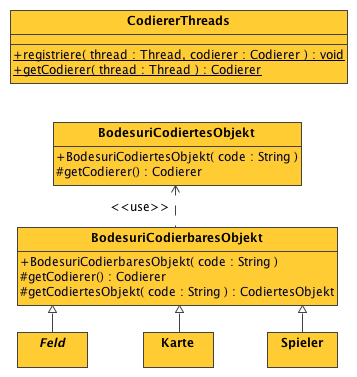
\includegraphics[width=0.7 \textwidth]{kd_pd_serialisierung}
	\caption{Klassendiagramm Serialisierung in PD}
	\label{fig:kd_pd_serialisierung}
\end{figure}


\clearpage
\subsection{Package dienste.automat}

Beinhaltet einen Zustandsautomaten der im Client und im Server für eine gezielte Abarbeitung des Spielablaufs sorgt. Der Automat wechselt aufgrund externer Events auf vorher definierten Bahnen zwischen den Zuständen hin und her.

Der Automat bietet zwei Betriebsmodi an:
\begin{itemize}
	\item Eigenständiger automatischer Betrieb in einem dedizierten Thread. Der Automat liest neue Ereignisse aus einer synchronisierten Queue und verarbeitet diese. Sind keine Ereignisse anstehend, blockiert der Automat.
	\item Ferngesteuerter integrierter Betrieb. Der Automat wird vom Caller bei anstehenden Ereignissen aufgerufen, verarbeitet exakt ein Ereignis (inklusive den dazugehörigen Zuständen) und übergibt anschliessend die Kontrolle wieder dem Caller. Der Modus eignet sich speziell für Unterautomaten bei welchen man keinen zusätzlichen Thread und eine seperate Ereignisqueue einsetzen möchte. Der Hauptautomat liest die Events ein und gibt sie direkt dem Unterautomaten weiter. 
\end{itemize}

\begin{figure}[H]
	\centering
	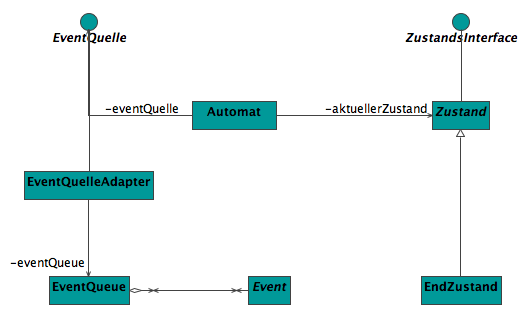
\includegraphics[width=0.7 \textwidth]{kd_dienste_automat}
	\caption{Klassendiagramm Automat}
	\label{fig:kd_dienste_automat}
\end{figure}

\paragraph{Schnittstellen}
\begin{itemize}
	\item Der Automat muss von den darüberliegenden Klassen abgeleitet und spezifisch implementiert werden.
\end{itemize}	

\clearpage
\subsection{Package dienste.serialisierung}

Dieses Package ist für die Serialisierung und Deserialisierung der Java-Objekte zuständig, die anschliessend über das Netzwerk versendet werden.

\paragraph{Schnittstellen}
\begin{itemize}
	\item Die abstrakte Klasse CodierbaresObjekt muss vom Benutzer dieses Packages implementiert werden. Dabei müssen die Methoden \texttt{getCodierer} und \texttt{getCodiertesObjekt} überschrieben werden. \texttt{getCodiertesObjekt} sollte ein neues konkretes CodiertesObjekt (z.\,B. BodesuriCodiertesObjekt) erstellen.
	\item Die zweite abstrakte Klasse CodiertesObjekt muss auch implementiert werden. Es muss nur \texttt{getCodierer} überschrieben werden, um den gleichen Codierer zurückzugeben wie bei CodierbaresObjekt.
\end{itemize}

\begin{figure}[H]
	\centering
	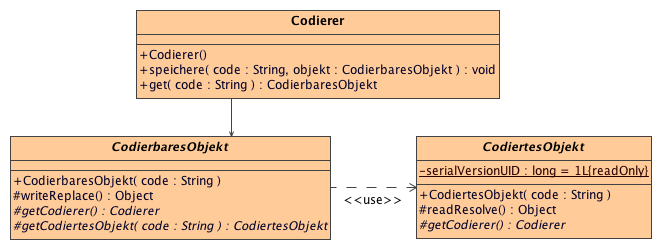
\includegraphics[width=\textwidth]{kd_dienste_serialisierung}
	\caption{Klassendiagramm Serialisierung in Dienste}
	\label{fig:kd_dienste_serialisierung}
\end{figure}

\clearpage
\subsection{Package dienste.netzwerk}

Dieses Package kapselt die Socket-Schnittstelle von Java und bietet Dienste für die Netzwerkkommunikation an.

\paragraph{Schnittstellen}
\begin{itemize}
	\item dienste.netzwerk verwendet das Interface \textbf{BriefkastenInterface} für die Kommunikation mit der darüberliegenden Schicht. Das \textbf{BriefkastenInterface} wird im Fall Bodesuri vom \textbf{BriefkastenAdaper} implementiert welches die eingehenden Nachrichten in eine EventQueue ablegt.
	\item Die Kommunikation mit dem Netzwerk findet über die Bibliotheken java.net statt.
\end{itemize}

\begin{figure}[H]
	\centering
	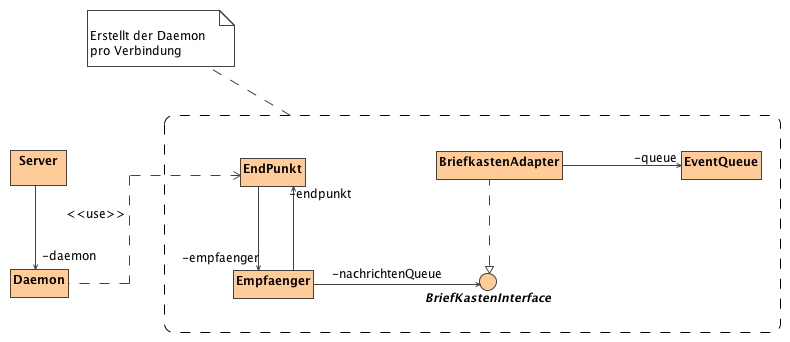
\includegraphics[width=0.5 \textwidth]{dienste_netzwerk_client}
	\caption{Klassendiagramm Client in Netzwerk}
	\label{fig:dienste_netzwerk_client}
\end{figure}

\begin{figure}[H]
	\centering
	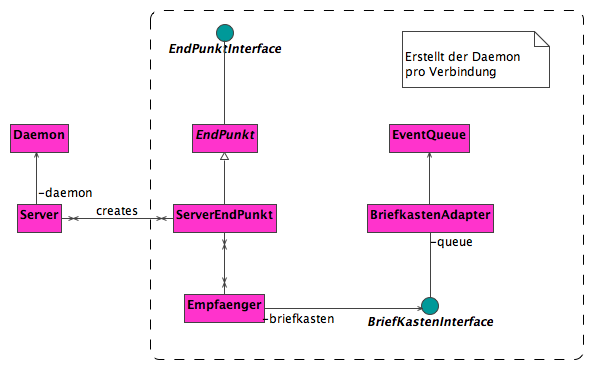
\includegraphics[width=0.9 \textwidth]{dienste_netzwerk_server}
	\caption{Klassendiagramm Server in Netzwerk}
	\label{fig:dienste_netzwerk_server}
\end{figure}

\clearpage
\subsection{Package ui}

Die UI-Schicht ist für die graphische Darstellung verantwortlich. Sie kommuniziert mit der Applikationsschicht top-down über direkte Assoziationen und bottom-up über Observer. Als weiteren wichtigen Bestandteil enthält die UI-Schicht auch den GUIController, welcher als Schnittstelle vom GUI zum Automaten agiert.

\paragraph{Übersicht der Views}
Die Abbildung~\vref{fig:views_uebersicht} stellt den Aufbau des GUIs dar. Das GUI besteht aus mehreren verschachtelten JPanels, welche in der Grafik gelb umrandet sind. Die blau umrandeten sind JLabels, welche für Texte und  Bilder verwendet wurden. Die einzelnen Grafiken werden mittels Koordinaten platziert, die in einem XML-Dokument erfasst sind und von der Klasse BrettXML ausgelesen werden.

\paragraph{JPanels (Views)}
Die gross geschriebenen Namen der Views sind zugleich Klassen, die von der Klasse JPanel ableiten.
\begin{enumerate}
	\item SpielView
	\item topPanel
	\item chatView
	\item BrettView
	\item SteuerungsView
	\item DeckView
	\item karteGewaehltView
	\item steuerungsView
\end{enumerate}

\paragraph{JLabels}
Die gross geschrieben Namen der JLabels sind zugleich Klassen, die von der Klasse BLabel ableiten. Die Klasse BLabel ist ebenfals eine abgeleitet Klasse von JLabel, sie ermöglicht das Zentrieren der Grafiken auf einem Koordinatenpunkt.

\begin{enumerate}
	\item hinweisLabel
	\item NormalesFeld2d
	\item SpielerFeld2d
	\item Figur2d
	\item spielerView
\end{enumerate}

\begin{figure}[H]
	\centering
	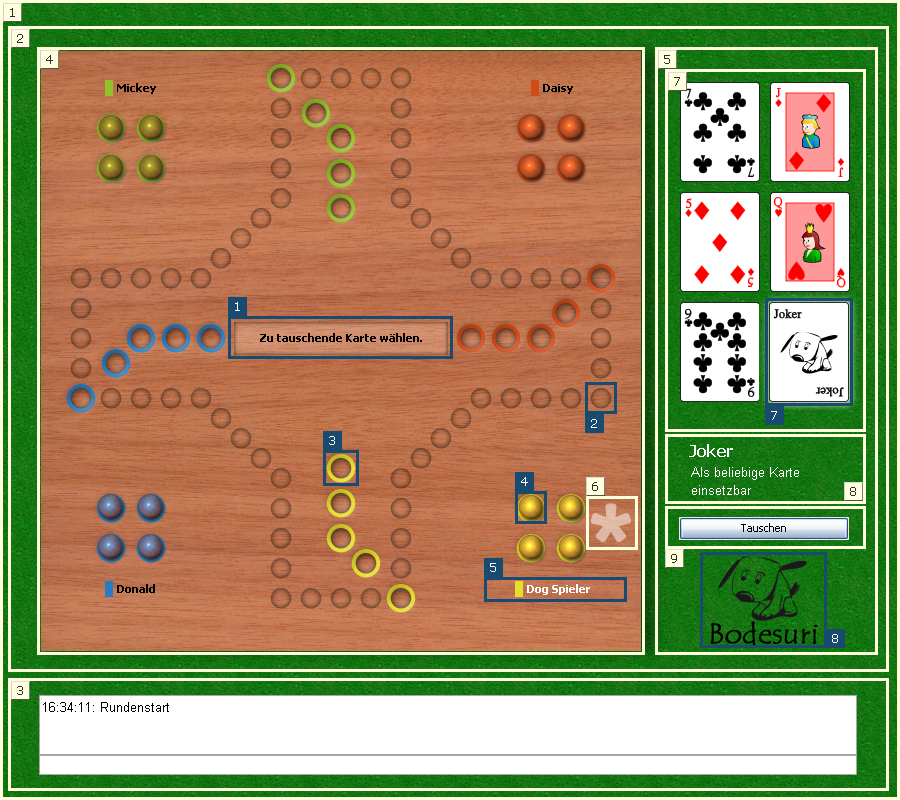
\includegraphics[width=\textwidth]{views_uebersicht}
	\caption{Übersicht der Views}
	\label{fig:views_uebersicht}
\end{figure}

\clearpage
\subsection{Package ui.geteiltes}

Dieses Package enthält Klassen, welche in verschiedenen Views verwendet werden. Sie dienen als Vereinheitlichung des Spielverhaltens.

\paragraph{Schnittstellen}
\begin{itemize}
	\item BLabel dient zur Positionierung der Labels zentriert auf einen Koordinatenpunkt.
	\item ClickMouseAdapter ist ein MouseListener, der das gleiche Klickverhalten wie ein ActionListener hat.
\end{itemize}

\subsection{Package ui.lobby}

In der Lobby werden die Spieler aufgelistet, die mit dem Server verbunden sind. Sobald sich alle vier Spieler in der Lobby befinden, kann das Spiel begonnen werden.

\subsection{Package ui.ressourcen}

Hier befinden sich die grafischen Ressourcen für das Spiel. Die einzelnen Grafiken werden von der Klasse Icons geladen und sind dann im gesamten Projekt über Konstanten erreichbar. Um die Grafiken per Koordinaten platzieren zu können, steht dafür ein XML-Dokument zur Verfügung, welches die Koordinaten der einzelnen Grafiken enthält. Anhand der Klasse BrettXML werden alle Koordinaten ausgelesen, um die Grafiken entsprechend zu platzieren.

\paragraph{Schnittstellen}
\begin{itemize}
	\item Icons dient zum Laden und Ansprechen der einzelnen Grafiken.
	\item BrettXML dient zum Auslesen der Koordinaten für die einzelnen Grafiken.
\end{itemize}

\subsection{Package ui.spiel}

Die Views des eigentlichen Spiels befinden sich in diesem Package. Sie sorgen für die Darstellung des Spielbrettes, sowie auch der Steuerung der Spielkarten und der Sonderfunktionen.

\begin{itemize}
	\item Das Package brett kümmert sich um die Darstellung des Spielbrettes, auf dem sich die Figuren, Felder und Spielernamen befinden.
	\item Das Package steuerung dient zum Ziehen der Karten und "<Tauschen"> der Spielkarten mit dem Partner oder das "<Aufgeben"> in einer Runde.
\end{itemize}

\begin{figure}[H]
	\centering
	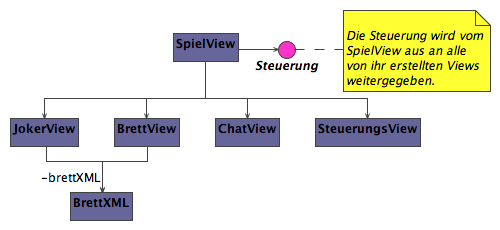
\includegraphics[width=0.8 \textwidth]{kd_ui_spiel}
	\caption{Klassendiagramm UI Spiel}
	\label{fig:kd_ui_spiel}
\end{figure}

\begin{figure}[H]
	\centering
	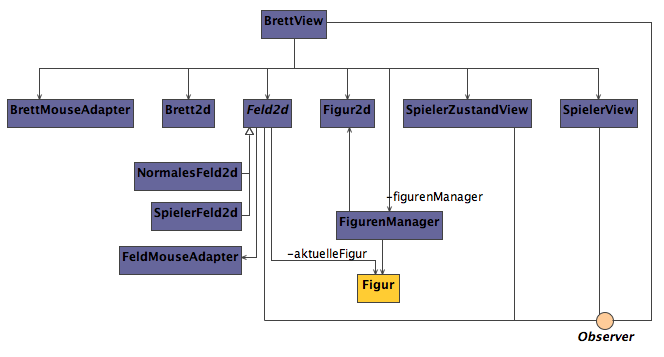
\includegraphics[width=0.7 \textwidth]{kd_ui_spiel_brett}
	\caption{Klassendiagramm UI Spiel Brett}
	\label{fig:kd_ui_spiel_brett}
\end{figure}

\begin{figure}[H]
	\centering
	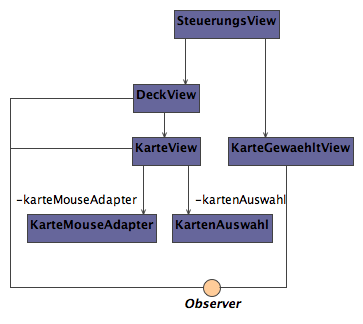
\includegraphics[width=0.5 \textwidth]{kd_ui_spiel_steuerung}
	\caption{Klassendiagramm UI}
	\label{fig:kd_ui_spiel_steuerung}
\end{figure}

\subsection{Package ui.verbinden}
Es regelt das kontrollierte Verbinden des Spielers zu einem angegebenen Server.

\begin{itemize}
	\item Die Aktion Abbrechen kümmert sich um das Schliessen des Frames.
	\item Die Aktion Beenden kümmert sich um das kontrollierte Beenden aller Threads.
	\item Die Aktion Verbinden kümmert sich um das Verbinden zum Server.
\end{itemize}

\begin{figure}[H]
	\centering
	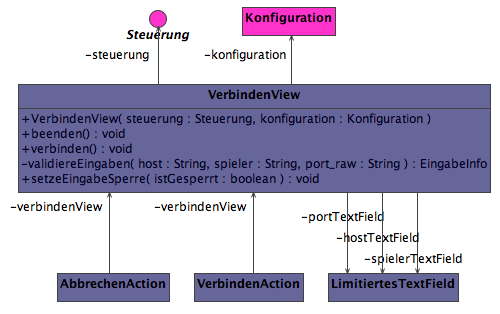
\includegraphics[width=0.7 \textwidth]{kd_ui_verbinden}
	\caption{Klassendiagramm UI}
	\label{fig:kd_ui_verbinden}
\end{figure}

\clearpage
\subsection{Package applikation}

Die Applikationsschicht ist für die Zustandssynchronisation (Spielstände usw.) verantwortlich.

\subsection{Package applikation.bot}
Zu Demonstration und Testzwecken wurde ein simpler Bot entwickelt. Dieser stellt für einen menschlichen Spieler keine Herausfoderung dar, er wählt aus allen möglichen Zügen, die ihm zur Verfügung stehen einen zufälligen aus und verfolgt somit keine gezielte Strategie.
	
\subsection{Package applikation.client}

	Die Client-Applikationsschicht ist für die Zustandsverwaltung des Clients und die Kommunikation mit dem UI verantwortlich. Die beiden Automaten (ClientAutomat \& ZugAutomat) und die clientspezifische PD bilden die Zustände des Clients ab. Der Controller dient als Kommunikationsschnittstelle zwischen dem Automaten und dem UI.
	
	\subsection{Package applikation.client.controller}

		Der Controller kanalisiert die Zugriffe der UI- auf die Applikationsschicht und umgekehrt. Andere Schichten nutzen bloss das Steuerungsinterface welches vom Controller implementiert wird.

		\paragraph{Schnittstellen}
		\begin{itemize}
			\item Der Controller bietet dem UI über das Steuerungs-Interface Methoden an um Events für den Automaten abzusetzen.
			\item Die abstrakten Methoden des Controllers (Methodennamen beginnen mit zeige), werden in der UI Schicht implementiert. Sie werden vom Automaten genutzt um das UI zu manipulieren.
		\end{itemize}

		\begin{figure}[H]
			\centering
			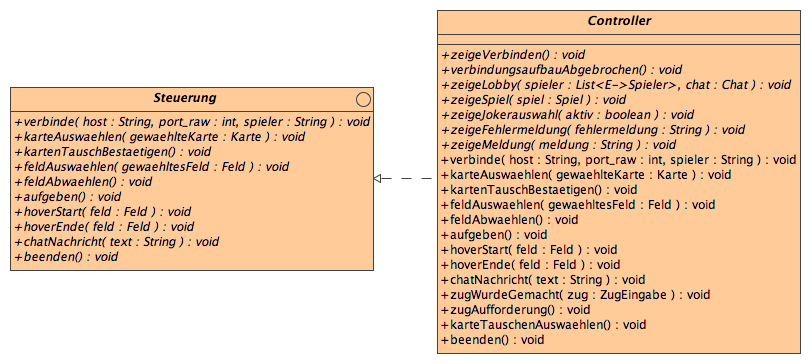
\includegraphics[width=\textwidth]{kd_client_controller}
			\caption{Klassendiagramm Controller}
			\label{fig:kd_client_controller}
		\end{figure}
		
	\subsection{Package applikation.client.events}

		Dieses Package beinhaltet die Events, die eintreten können und um deren Behandlung sich der Automat kümmert.
		\begin{figure}[H]
			\centering
			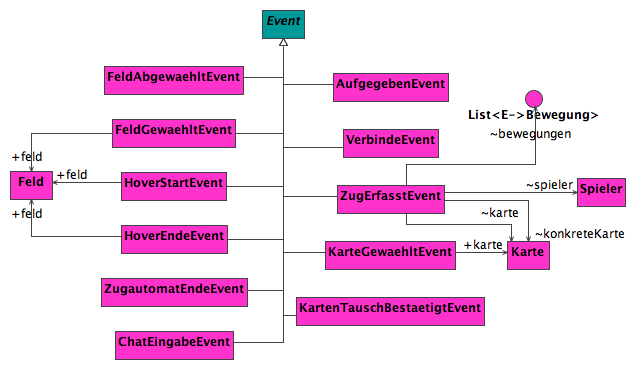
\includegraphics[width=\textwidth]{kd_client_events}
			\caption{Klassendiagramm Events}
			\label{fig:kd_client_events}
		\end{figure}
		
	\subsection{Package applikation.client.konfiguration}

		Beinhaltet Standardwerte und Debugeinstellungen für die Konfiguration des Clients.	

		\subparagraph{Schnittstellen}
		\begin{itemize}
			\item Werden in der clientspezifischen PD gespeichert und dann vom Automaten, dem Controller und dem UI genutzt.
		\end{itemize}
	
	\subsection{Package applikation.client.pd}

		Die clientspezifische PD erweitert die PD um zustandsabhängige Eigenschaften.

		\paragraph{Schnittstellen}
		\begin{itemize}
			\item Die clientspezifische PD bietet eine Teilmenge der Funktionen der PD sowie einige zusätzliche Funktionen an. Einstiegspunkt ist das Spiel, da es die Spieler, das Brett und die Karten enthält.
			\item Die Felder, die Karten, die Spieler und das Spiel sind \emph{Observeable}.
		\end{itemize}

		\begin{figure}[H]
			\centering
			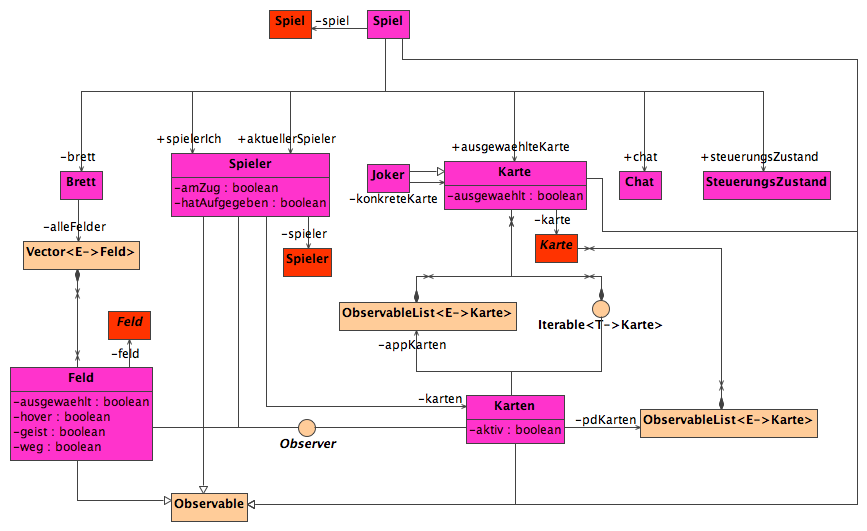
\includegraphics[width=0.7 \textwidth]{kd_client_pd}
			\caption{Klassendiagramm clientspezifische PD}
			\label{fig:kd_client_pd}
		\end{figure}
		
	\subsection{Package applikation.client.zugautomat}

		Ein eigener Automat inklusive einer kleinen clientspezifischen PD. Wird jede Runde für die Erfassung eines Zuges vom ClientAutomaten gestartet und gibt dem Automaten einen fertig erfassten Zug zurück.

		\paragraph{Schnittstellen}
		\begin{itemize}
			\item Der Zugautomat kommuniziert über Events mit dem ClientAutomaten.
		\end{itemize}
		
		\begin{figure}[H]
			\centering
			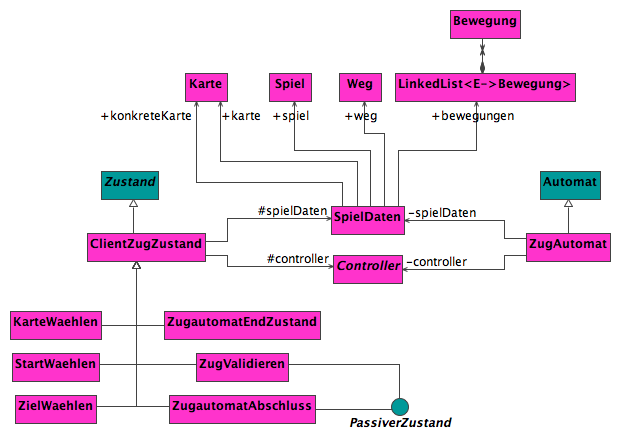
\includegraphics[width=\textwidth]{kd_client_zugautomat}
			\caption{Klassendiagramm der Zugerfassung}
			\label{fig:kd_client_zugautomat}
		\end{figure}
		
	\subsection{Package applikation.client.zustaende}

		Dieses Package gruppiert die Zustände die der ClientAutomat annehmen kann.

		\paragraph{Schnittstellen}
		\begin{itemize}
			\item Die Zustände werden vom ClientAutomaten genutzt.
		\end{itemize}
		
		\begin{figure}[H]
			\centering
			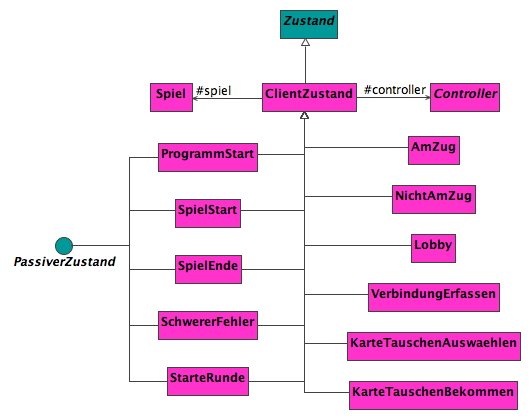
\includegraphics[width=\textwidth]{kd_client_zustaende}
			\caption{Klassendiagramm Zustände des Clients}
			\label{fig:kd_client_zustaende}
		\end{figure}
	
\subsection{Package applikation.nachrichten}

	Dieses Package beinhaltet alle möglichen Nachrichtentypen, die zur Kommunikation zwischen Client und Server verwendet werden. Alle Nachrichten Müssen von der Basisklasse Nachricht ableiten.
	
	Eine Liste der Nachrichten kann unter \vref{sub:nachrichten}

\subsection{Package applikation.server}

	Der Zustandsautomat des Servers und dessen Zustände. Sorgt für den korrekten Ablauf des Spiels auf der Server-Seite. Verarbeitet die eintretenden Events vom Netzwerk und löst entsprechende Aktionen aus, um den Spielablauf zu steuern.

	\begin{figure}[H]
		\centering
		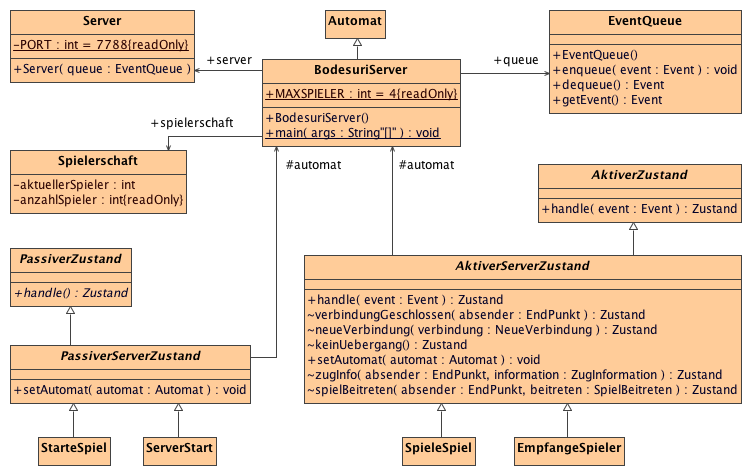
\includegraphics[width=0.5 \textwidth]{kd_applikation_server}
		\caption{Klassendiagramm Server in Applikation}
		\label{fig:kd_applikation_server}
	\end{figure}
	
	\subsection{Package applikation.server.pd}

		\begin{figure}[H]
			\centering
			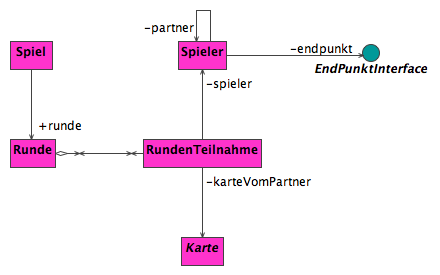
\includegraphics[width=0.5 \textwidth]{kd_server_pd}
			\caption{Klassendiagramm serverspezifische PD}
			\label{fig:kd_server_pd}
		\end{figure}

		\paragraph{Schnittstellen}
		\begin{itemize}
			\item Die serverspezfische PD bietet eine Teilmenge der Funktionen der PD sowie einige zusätzliche Funktionen an.
		\end{itemize}

\clearpage
\section{Prozesse \& Threads}
Ein reguläres Bodesuri-Spiel besteht aus fünf eigenständigen Komponenten. Dies sind die vier Clients und der zentrale Server. Zwischen den Clients und dem Server besteht je ein TCP Socket. 

\begin{figure}[h]
	\centering
	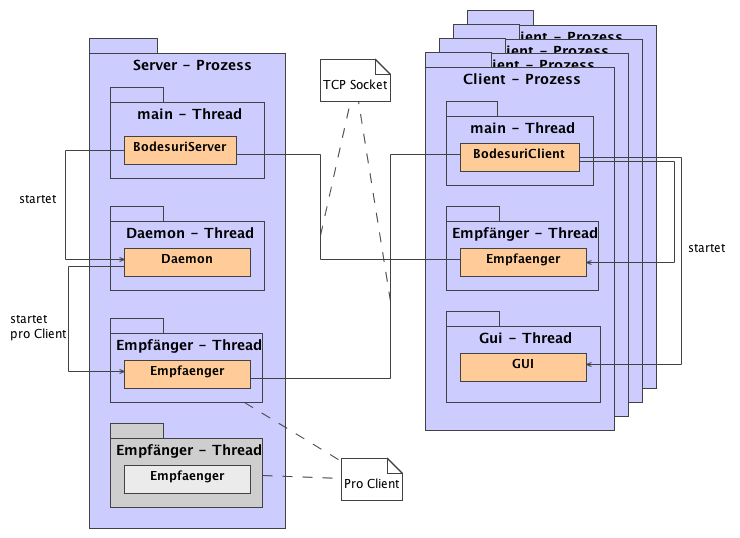
\includegraphics[width=\textwidth]{prozesse_und_threads}
	\caption{Prozesse \& Threads}
	\label{fig:prozesse_und_threads}
\end{figure}

\clearpage
\subsection{Client-Threads}
\label{ssub:client_threads}

\paragraph{Main-Thread}
\label{ssub:main_thread}

Der Main-Thread des Clients ist für die geordnete Koordination zwischen dem Spieler (via GUI) und den anderen Clients (via Server) zuständig.


\begin{tabular}{@{} l p{12.5cm}}
\textbf{Klasse}       & BodesuriClient \\
\textbf{Anzahl}       & 1 \\
\textbf{Gestartet}    & Bei Prozessbeginn \\
\textbf{Beendet}      & Bei Programmende
\end{tabular}

\paragraph{Empfänger-Thread}

Der Empfänger-Thread ist für den Empfang von Netzwerk-Nachrichten zuständig. Er liest aus einem java.net.Socket und speichert die eingegangenen Nachrichten über das Briefkasten-Interface in der EventQueue.

\begin{tabular}{@{} l p{12.5cm}}
\textbf{Klasse}       & Empfaenger \\
\textbf{Anzahl}       & 1 \\
\textbf{Gestartet}    & Bei Verbindungsaufbau durch den Main-Thread (Klasse Endpunkt) \\
\textbf{Beendet}      & Bei Verbindungsabbau durch den Main-Thread (Klasse Endpunkt) oder bei Fehlern selbständig.
\end{tabular}


\paragraph{Swing-Threads}
\label{ssub:swing_threads}

Swing startet intern verschiedene Threads. Die genauen Abläufe und Struktur dieser Threads sind für diese Dokumentation nicht relevant.

\begin{tabular}{@{} l p{12.5cm}}
\textbf{Klasse}       & AWK-AppKit \\
\textbf{Anzahl}       & 1..* \\
\textbf{Gestartet}    & Durch Swing \\
\textbf{Beendet}      & N/A


\end{tabular}

\clearpage
\subsection{Server Threads}
\label{ssub:server}

Der Server ist für die Koordination der einzelnen Clients zuständig.

\begin{tabular}{@{} l p{12.5cm}}
\textbf{Klasse}       & BodesuriServer \\
\textbf{Anzahl}       & 1 \\
\textbf{Gestartet}    & bei Prozessbeginn \\
\textbf{Beendet}      & Bei Spielende oder bei schweren Fehlern
\end{tabular}

\paragraph{Daemon}
\label{ssub:daemon}

Der Daemon ist ein Teil des Servers. Er nimmt eingehende Verbindungen entgegen und meldet diese über das BriefkastenInterface (via EventQueue) an den Nutzer des Servers.

\begin{tabular}{@{} l p{12.5cm}}
\textbf{Klasse}       & Daemon \\
\textbf{Anzahl}       & 1 \\
\textbf{Gestartet}    & Durch den Main-Thread (Klasse Server) gestartet \\
\textbf{Beendet}      & Bei Programmende
\end{tabular}

\paragraph{Empfänger-Thread}

Der Empfänger-Thread ist für den Empfang von Netzwerk-Nachrichten zuständig. Er liest aus einem java.net.Socket und speichert die eingegangenen Nachrichten über das Briefkasten-Interface in der EventQueue.

Es wird pro offene Verbindung ein Empfänger gestartet.

\begin{tabular}{@{} l p{12.5cm}}
\textbf{Klasse}       & Empfänger \\
\textbf{Anzahl}       & 1..4 \\
\textbf{Gestartet}    & Durch den Daemon bei eingehenden Verbindungen  \\
\textbf{Beendet}      & Bei Verbindungsabbau durch den Main-Thread
\end{tabular}

\clearpage
\section{Spielablauf \& -zustände}

Das Spiel verfügt über einen komplexen Ablauf, den wir mit Hilfe eines Zustandsautomaten implementiert haben. Nachfolgend werden die Automaten für den Client und den Server inklusive der Events erklärt.

\subsection{Zustände Client}

Abbildung~\vref{fig:zd_applikation_bodesuriclient} zeigt den Ablauf der Zustände des Clients. Zustände in grün sind passive Zustände.
\begin{figure}[h]
	\centering
	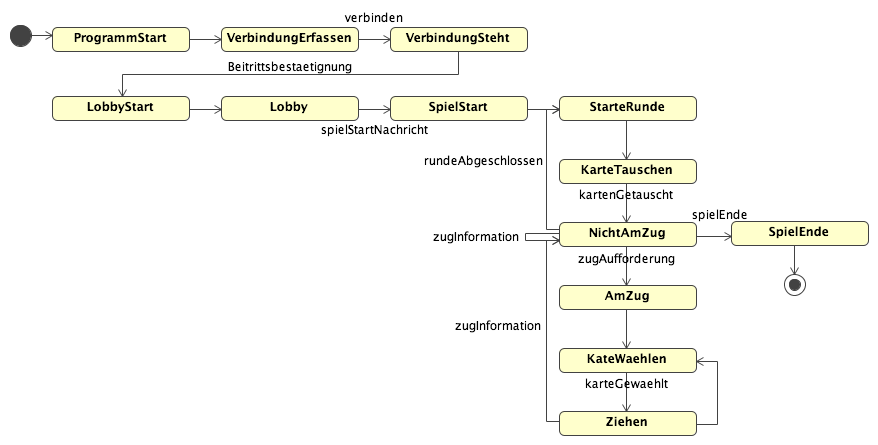
\includegraphics[width=\textwidth]{zd_applikation_bodesuriclient}
	\caption{Zustandsdiagramm Client}
	\label{fig:zd_applikation_bodesuriclient}
\end{figure}

\subsubsection{ProgrammStart}
\label{ssub:programmstart}
Zustand in welchem der Automat beim Start ist. Öffnet den \textbf{VerbindenView} und geht direkt in den Zustand \textbf{VerbindungErfassen} über.


\subsubsection{VerbindungErfassen}
\label{ssub:verbinungerfassen}
Zustand wenn der Spieler die Verbindungsdaten eingeben muss. Wenn ein \textbf{VerbindeEvent} eintrifft, wird der Zustand \textbf{Lobby} aufgerufen.

\subsubsection{Lobby}
\label{ssub:lobby}
Zustand wenn der Spieler in der Lobby ist.
\begin{itemize}
	\item Wenn eine \textbf{SpielStartNachricht} eintrifft, wird der Zustand \textbf{SpielStart} aufgerufen.
	\item Wenn eine \textbf{BeitrittsInformation} eintrifft, werden die Informationen über die beigetretenen Spieler aktualisiert. Der Zustand wird nicht gewechselt.
	\item Wenn eine \textbf{BeitrittVerweigertNachricht} eintrifft, wird das Spiel beendet.
\end{itemize}

\subsubsection{SpielStart}
\label{ssub:spielstart}
Zustand in welchem das Spiel (\textbf{BodesuriView}) gestartet wird. Geht direkt in \textbf{NichtAmZug} über.

\subsubsection{NichtAmZug}
\label{ssub:nichtamzug}
Zustand wenn der Spieler nicht am Zug ist.
\begin{itemize}
	\item 	Wenn eine \textbf{ZugAufforderung} eintrifft, wird der Zustand \textbf{AmZug} aufgerufen.
	\item 	Wenn eine \textbf{AktuellerSpielerInformation} eintrifft, wird der aktuelle Spieler dargestellt, der Zustand aber nicht gewechselt.
	\item 	Wenn eine \textbf{ZugEingabe} eintrifft, wird Zug aus der Eingabe visualisiert. Der Zustand wird nicht gewechselt.
	\item 	Wenn eine \textbf{RundenStart}-Nachricht eintrifft, werden die erhaltenen Karten gespeichert und der Zustand \textbf{StarteRunde} aufgerufen.
	\item 	Wenn eine \textbf{AufgabeInformation} eintrifft, wird der Spieler, welcher aufgegeben hat, im UI angepasst. Der Zustand wird nicht gewechselt.
	\item 	Wenn eine \textbf{SpielFertigNachricht} eintrifft, wird der Gewinner angezeigt und \textbf{SpielEnde} aufgerufen.
\end{itemize}

\subsubsection{StarteRunde}
\label{ssub:starterunde}
Zustand wenn eine neue Runde gestartet wird. Alle Eigenschaften der Spieler werden zurückgesetzt. Der Automat geht nach \textbf{KarteTauschenAuswaehlen} über.

\subsubsection{KarteTauschenAuswaehlen}
\label{ssub:kartetauschenauswaehlen}
Zustand in dem wir warten bis der Spieler die Karte, die er tauschen möchte, ausgewählt hat. Tritt \textbf{KarteGewaehltEvent} ein, gehen wir in den Zustand \textbf{KarteTauschenBekommen} über.

\subsubsection{KarteTauschenBekommen}
\label{ssub:kartetauschenbekommen}
Zustand wenn wir auf die Karte, die wir von unserem Mitspieler erhalten, warten. Wenn sie eintrifft, wird der Zustand \textbf{NichtAmZug} aufgerufen.

\subsubsection{AmZug}
\label{ssub:amzug}
Zustand in welchem der Spieler am Zug ist. Erstellt einen \textbf{ZugAutomaten}, der sich um das Erfassen und Validieren eines Zuges kümmert. Eintreffende Events werden direkt an den \textbf{ZugAutomaten} weitergeleitet. Dieser sendet einen \textbf{ZugErfasstEvent} wenn er fertig ist. Der Event wird versandt und der Automat geht nach \textbf{NichtAmZug} über.

\subsubsection{SpielEnde}
Zustand in welchem sich dem Automat befindet wenn wir das Spiel beenden wollen. In diesem Zustand werden Events, die möglicherweise noch in der Queue warten, konsumiert, das UI heruntergefahren, die Verbindung zum Server geschlossen und der Automat beendet.

\subsection{Zustände ZugAutomat}
\label{sub:zustände_zugautomat}
Die Erfassung eines Zuges wurde aus dem Client-Automaten ausgelagert. Abbildung~\vref{fig:zd_applikation_bodesuriserver} zeigt den Ablauf der Zustände des \textbf{ZugAutomat}. Zustände in grün sind passive Zustände.
\begin{figure}[h]
	\centering
	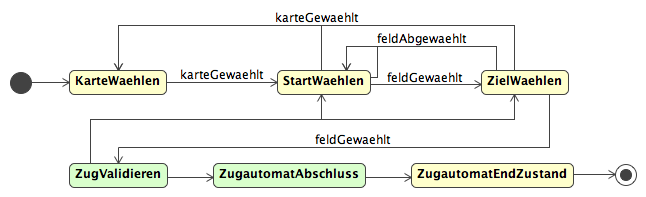
\includegraphics[width=\textwidth]{zd_applikation_zugautomat}
	\caption{Zustandsdiagramm ZugAutomat}
	\label{fig:zd_applikation_zugautomat}
\end{figure}

\subsubsection{KarteWaehlen}
\label{ssub:kartewaehlen}
Zustand wenn der Spieler eine Karte auswählen muss. Wenn der \textbf{KarteGewaehltEvent} eintritt, wird der Zustand \textbf{StartWaehlen} aufgerufen.

\subsubsection{StartWaehlen}
\label{ssub:startwaehlen}
Zustand wenn der Spieler das Startfeld wählen muss.
\begin{itemize}
	\item Trifft ein \textbf{FeldGewaehltEvent} ein, wird das Feld überprüft. Ergibt die Wahl Sinn, wird nach \textbf{ZielWaehlen} gewechselt. Sonst bleiben wir in diesem Zustand.
	\item Trifft ein \textbf{KarteGewaehltEvent} ein (der Spieler hat eine andere Karte ausgewählt) wird nach \textbf{KarteWaehlen} gewechselt.
	\item Trifft ein \textbf{FeldAbgewaehltEvent} ein, wird das Brett zurückgesetzt. Wir bleiben aber in diesem Zustand.
\end{itemize}

\subsubsection{ZielWaehlen}
\label{ssub:zielwaehlen}
Zustand wenn der Spieler das Zielfeld wählen muss.
\begin{itemize}
	\item Trifft ein \textbf{FeldGewaehltEvent} ein, wird das Feld überprüft. Ergibt die Wahl Sinn, wird nach \textbf{ZugValidieren} gewechselt. Wurde das Startfeld ausgewählt, wird das Startfeld wieder deaktiviert und nach \textbf{StartWaehlen} gewechselt.
	\item Trifft ein \textbf{KarteGewaehltEvent} ein (der Spieler hat eine andere Karte ausgewählt), wird nach \textbf{KarteWaehlen} gewechselt.
	\item Trifft ein \textbf{FeldAbgewaehltEvent} ein, wird das Brett zurückgesetzt. Wir bleiben aber in diesem Zustand.
	\item \textbf{HoverStartEvent} und \textbf{HoverEndeEvent} aktiveren bzw. deaktivieren das Hervorheben des Weges.
\end{itemize}

\subsubsection{ZugValidieren}
\label{ssub:zugvalidieren}
Validiert den erfassten Zug.
\begin{itemize}
	\item Ist die Karte eine Sieben und es wurden noch keine 7 Felder gefahren, wechseln wir zurück nach \textbf{StartWaehlen} um eine weitere Bewegung zu erfassen.
	\item Ist der Zug ungültig, wird eine Fehlermeldung gezeigt und zurück nach \textbf{ZielWaehlen} gewechselt.
	\item Ist der Zug gültig, wird er zurück an den \textbf{ClientAutomat} übermittelt und nach \textbf{ZugautomatAbschluss} gewechselt.
\end{itemize}

\subsubsection{ZugautomatAbschluss}
\label{ssub:zugautomatabschluss}
Räumt den Zugautomaten auf. Alle Bewegungen werden zurückgesetzt, die Kartenauswahl deaktiviert, die \textbf{SteuerungsButtons} ausgeblendet und in \textbf{ZugautomatEndZustand} übergegangen.

\subsubsection{ZugautomatEndZustand}
\label{ssub:zugautomatendzustand}
Endzustand des Zugautomaten. Ignoriert alle eingehenden Events.


\subsection{Zustände Server}
\label{sub:zustände_server}

Abbildung~\vref{fig:zd_applikation_bodesuriserver} zeigt den Ablauf der Zustände des Servers.

\begin{figure}[h]
	\centering
	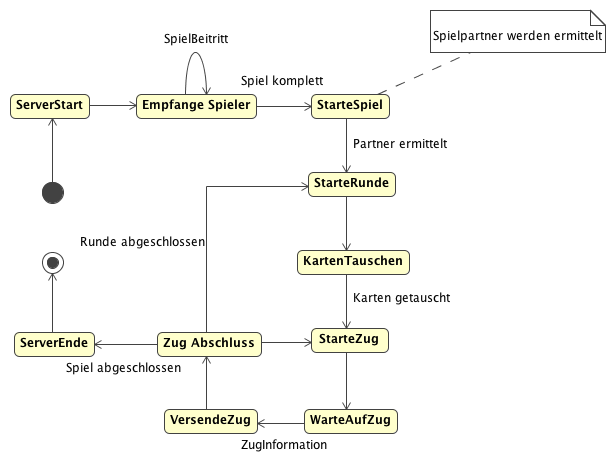
\includegraphics[width=\textwidth]{zd_applikation_bodesuriserver}
	\caption{Zustandsdiagramm Server}
	\label{fig:zd_applikation_bodesuriserver}
\end{figure}

\subsubsection{ServerStart}
\label{ssub:serverStart}
Server wird gestartet. Der TCP-Daemon wird initialisiert und es werden die notwendigen Vorbereitungen getroffen um Spieler zu akzeptieren. Geht direkt in den Zustand \textbf{EmpfangeSpieler} über.

\subsubsection{EmpfangeSpieler}
\label{ssub:empfangespieler}
Der Server empfängt solange neue Spieler bis das Spiel vollzählig ist.

Erhält der Server die Nachricht \textbf{SpielBeitreten} prüft er ob bereits ein Spieler dem angegebenen Namen im Spiel vorhanden ist. Falls nicht, bestätigt er den Beitritt mit der Nachricht \textbf{SpielBeitreten} und informiert die restlichen Spieler über den Neuling mit der Nachricht \textbf{BeitrittsInformation}

Sobald alle Spieler komplett sind, wird in den Zustand \textbf{SpielStart} gewechselt.

\subsubsection{SpielStart}
\label{ssub:startespiel}
Den Spielern wird der Spielstart mit der Nachricht \textbf{SpielStartNachricht} angekündet. Die Partnerschaften werden, wie auf Abbildung~\vref{fig:dienste_partner} gezeigt, zwischen den Spielern ausgehandelt.\footnote{Wurde nicht implementiert.}

Die Nachricht \textbf{SpielStartNachricht} enthält die Namen aller Spieler und die gebildeten Partnerschaften.

Geht direkt in den Zustand \textbf{StartRunde} über.

\subsubsection{StartRunde}
\label{ssub:startrunde}
Eine neue Runde wird gestartet und mit der Nachricht \textbf{RundenStart} den Spielern mitgeteilt. Es werden allen Spielern Karten ausgeteilt.

\subsubsection{KartenTauschen}
\label{ssub:kartentauschen}
Alle Spieler müssen mit ihrem Partner eine Karte tauschen. Der Server wartet bis alle Spieler die zu tauschende Karte mit der Nachricht \textbf{KartenTausch} gemeldet haben. Anschliessend wird die getauschte Karte mit derselben Nachricht dem Partner gemeldet und es wird in den Zustand \textbf{StarteZug} gewechselt.

\subsubsection{StarteZug}
\label{ssub:startezug}
Ein neuer Zug wird gestartet. Hierfür bestimmt der Server zuerst wer an der Reihe ist und teilt dies dem betroffenen Spieler mittels der Nachricht \textbf{ZugAufforderung} mit. 

Die restlichen Spielern werden mit der Nachricht \textbf{AktuellerSpielerInformation} darüber informiert wer gerade am Zug ist.

Anschliessend wird direkt in den Zustand \textbf{WarteAufZug} gewechselt.

\subsubsection{WarteAufZug}
\label{ssub:warteaufzug}
Der Server wartet, bis der \textbf{Spieler} seinen \textbf{Zug} erfasst hat. Der Spieler kann entweder den erfassten \textbf{Zug} mittels der Nachricht \textbf{ZugInformation} melden oder mittels der Nachricht \textbf{Aufgabe} aufgeben. Die restlichen Spieler werden über die durchgeführte Aktion informiert.

Hat der Spieler aufgegeben oder keine Karten mehr wird er aus der aktuellen \textbf{Runde} entfernt.

Hat der Server eine Spieler-Reaktion erhalten, sei es \textbf{ZugInformation} oder Aufgaben, wird in den Zustand \textbf{ZugAbschluss} gewechselt.

\subsubsection{ZugAbschluss}
\label{ssub:zugabschluss}
Server schliesst den Zug formell ab. Es wird geprüft, ob das Spiel beziehungsweise die Runde abgeschlossen ist und in den Zustand \textbf{ServerStoppen} respektive \textbf{StartRunde} gewechselt. Ist weder das Spiel noch die Runde fertig wird in den Zustand \textbf{StarteZug} gewechselt.

Bei Spielende wird der Gewinner mittels der Nachricht \textbf{SpielFertigNachricht} allen Spielern mitgeteilt.
	
\subsubsection{ServerStoppen}
Es wird geprüft ob noch irgendwelche \textbf{Spieler} mit dem Server verbunden sind. Ist dies der Fall wird in den Zustand \textbf{WarteBisAlleVerbindungenWeg} gewechselt. Ansonsten wird der \textbf{ServerAutomat} in den \textbf{Endzustand} überführt und beendet sich selber.

\subsubsection{WarteBisAlleVerbindungenWeg}

Der Server wartet bis alle verbleibenden Verbindungen beendet sind. Sobald dies der Fall ist wird der \textbf{ServerAutomat} in den \textbf{Endzustand} überführt und beendet sich selber.

\clearpage
\subsection{Nachrichten}
\label{sub:nachrichten}

Die folgenden Nachrichten dienen der Kommunikation zwischen Client und Server und lösen in den Automaten Zustandsübergänge aus.

\begin{itemize}
	\item AktuellerSpielerInformation
	\item Aufgabe
	\item AufgabeInformation
	\item BeitrittVerweigert
	\item BeitrittsInformation
	\item ChatNachricht
	\item KartenTausch
	\item RundenStart
	\item SpielAbbruch
	\item SpielBeitreten
	\item SpielFertigNachricht
	\item SpielInfo
	\item SpielStartNachricht
	\item SpielerInfo
	\item ZugAufforderung
	\item ZugInformation
\end{itemize}


\clearpage
\section{Dynamische Abläufe}

Mit den nachfolgenden Sequenzdiagrammen wollen wir die Abläufe zwischen den Schichten sowie zeitliche Abläufe aufzeigen.

\subsection{Nachrichtenfluss durch die Schichten}

Die Abbildungen~\vref{fig:sd_verbindung_erstellen_client} und~\vref{fig:sd_verbindung_erstellen_server} zeigen den Schnitt durch die Architektur von Bodesuri. Sie zeigen die Aufrufe durch die Architekturschichten beim Erstellen einer neuen Verbindung auf der Seite des Clients und des Servers.
\begin{figure}[h]
	\centering
	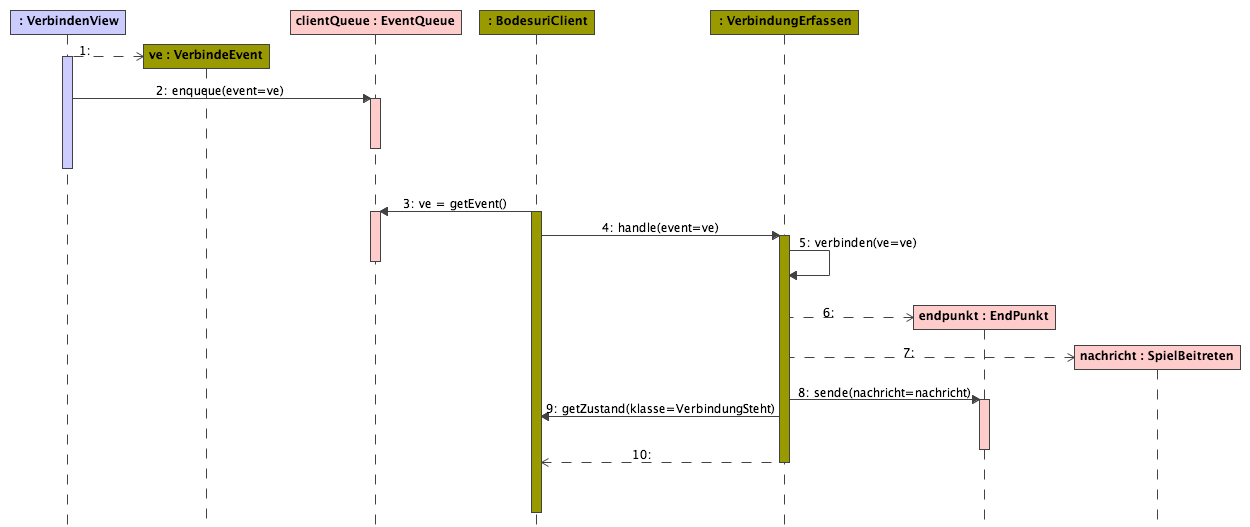
\includegraphics[width=\textwidth]{sd_verbindung_erstellen_client}
	\caption{Sequenzdiagramm Verbindung erstellen -- Client}
	\label{fig:sd_verbindung_erstellen_client}
\end{figure}
\begin{figure}[h]
	\centering
	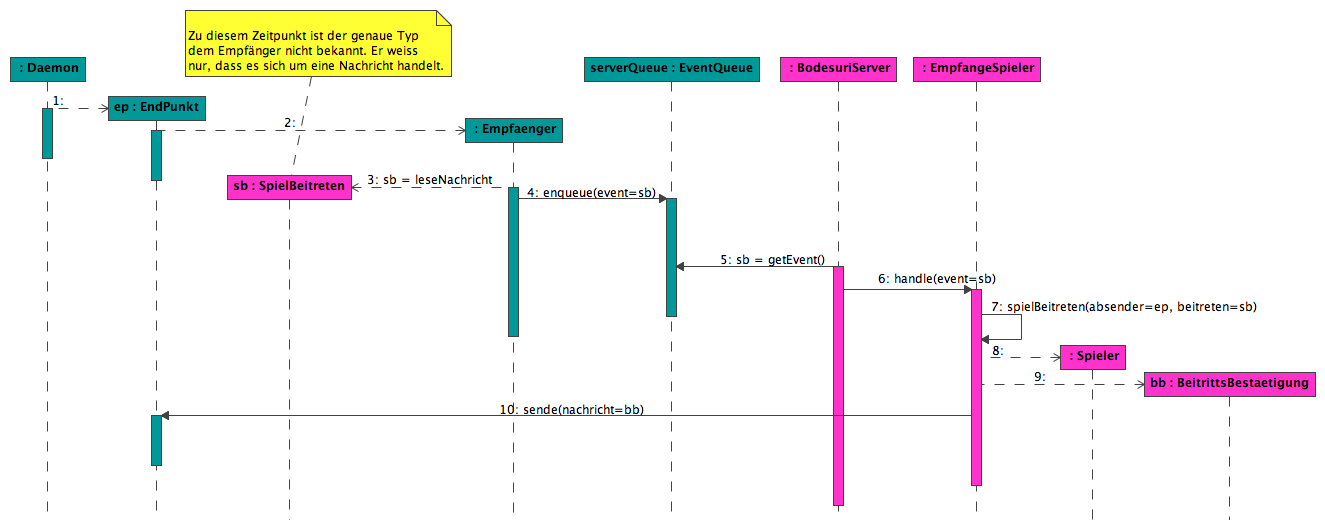
\includegraphics[width=\textwidth]{sd_verbindung_erstellen_server}
	\caption{Sequenzdiagramm Verbindung erstellen -- Server}
	\label{fig:sd_verbindung_erstellen_server}
\end{figure}

\begin{figure}[h]
	\centering
	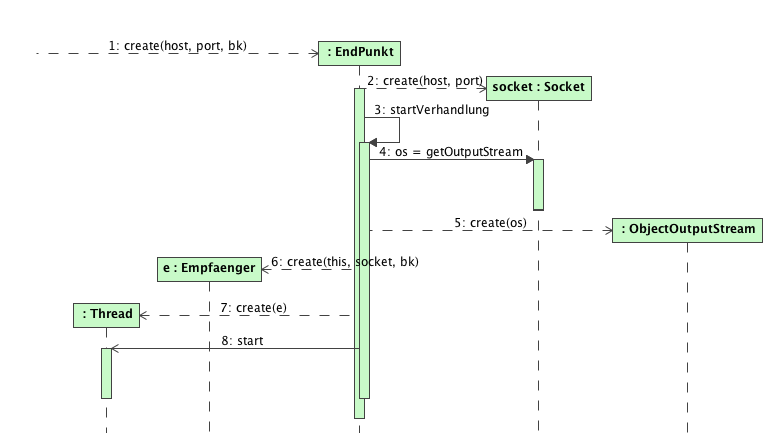
\includegraphics[width=\textwidth]{sd_verbindung_erstellen_endpunkt}
	\caption{Sequenzdiagramm Verbindung erstellen -- EndPunkt}
	\label{fig:sd_verbindung_erstellen_endpunkt}
\end{figure}

\subsection{Rundenstart}
\label{sub:rundenstart}
Die Abbildung~\vref{fig:dienste_rundenstart} zeigt den Ablauf beim Start einer neuen Runde.
\begin{figure}[h]
	\centering
	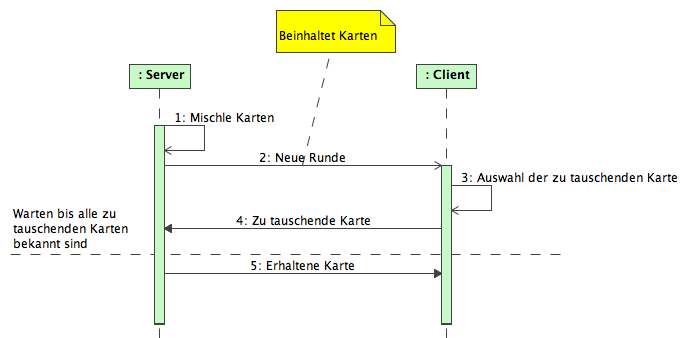
\includegraphics[width=0.7 \textwidth]{dienste_rundenstart}
	\caption{Sequenzdiagramm Rundenstart}
	\label{fig:dienste_rundenstart}
\end{figure}

\clearpage
\subsection{Validierung von Spielzügen}
\label{ssub:validierung_von_spielzügen}
Abbildung~\vref{fig:pd_validierung} zeigt die Validierung der Spielzüge.
\begin{figure}[h]
	\centering
	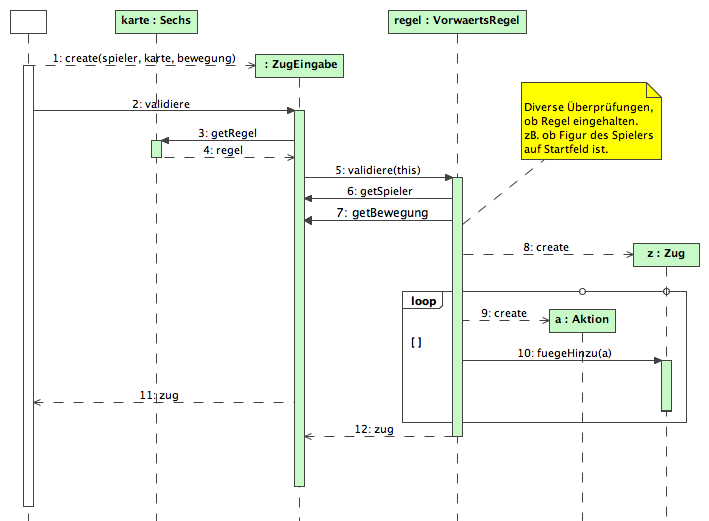
\includegraphics[width=\textwidth]{pd_validierung}
	\caption{Sequenzdiagramm Validierung von Spielzügen}
	\label{fig:pd_validierung}
\end{figure}

\clearpage
\subsection{Serialiserung}
\label{sub:serialiserung}
Abbildung~\vref{fig:dienste_serialisierung} zeigt den Ablauf bei der Serialisierung von Objekten, damit sie über das Netzwerk übertragen werden können.
\begin{figure}[h]
	\centering
	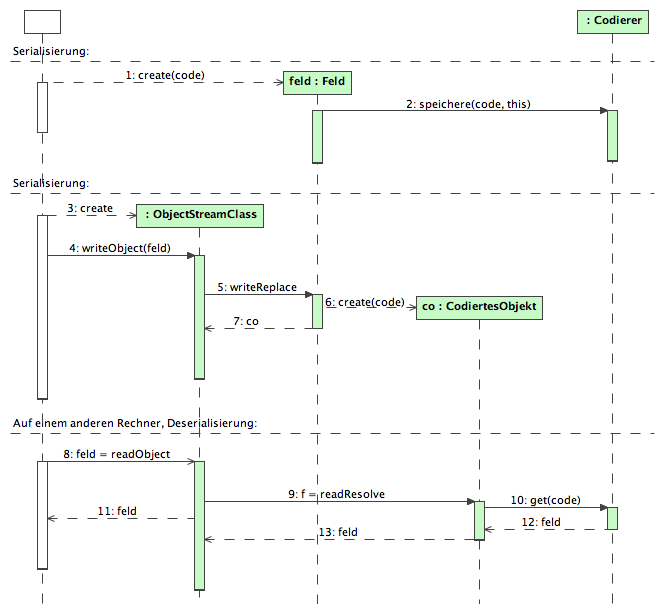
\includegraphics[width=\textwidth]{dienste_serialisierung}
	\caption{Sequenzdiagramm Serialisierung}
	\label{fig:dienste_serialisierung}
\end{figure}

\clearpage

\subsection[Partnerschaften bilden]{Partnerschaften bilden\footnote{Wurde nicht implementiert.}}
\label{sub:partnerschaften_bilden}

Abbildung~\vref{fig:dienste_partner} zeigt die möglichen Zustände beim Finden eines Partners.
\begin{figure}[h]
	\centering
	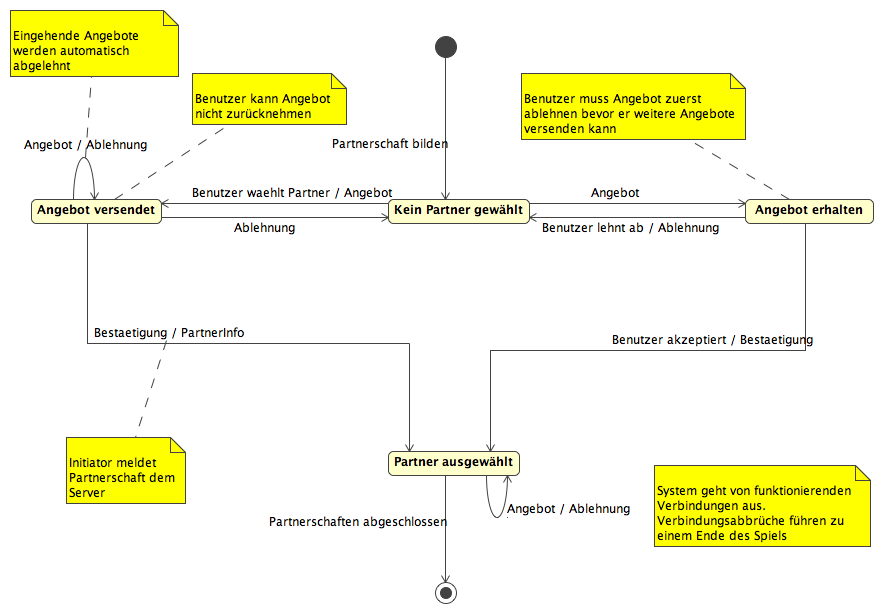
\includegraphics[width=\textwidth]{dienste_partner}
	\caption{Zustandsdiagramm Partnerschaften bilden}
	\label{fig:dienste_partner}
\end{figure}

Die Abildung~\vref{fig:dienste_partnerschaft_normal} zeigt Ablauf des Bildens von Partnerschaften.
\begin{figure}[h]
	\centering
	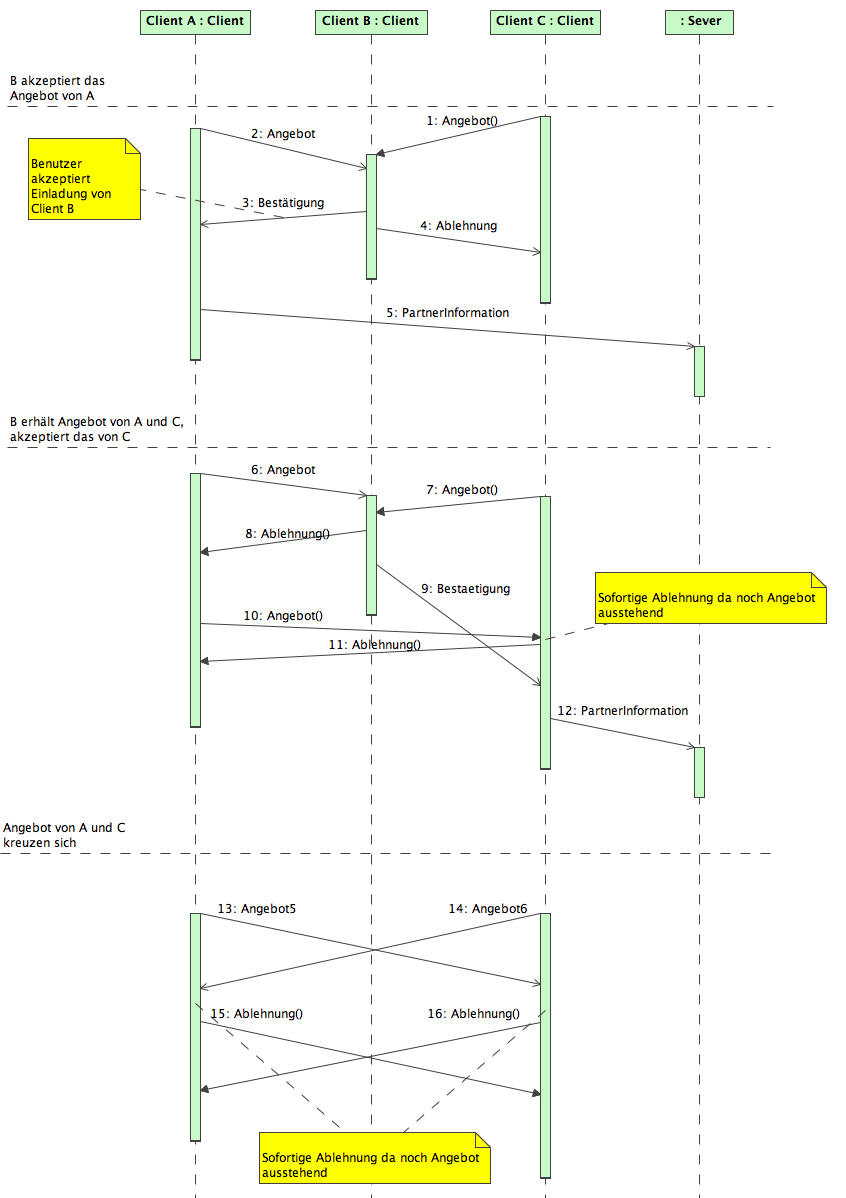
\includegraphics[width=\textwidth]{dienste_partnerschaft_normal}
	\caption{Sequenzdiagramm Partnerschaften bilden}
	\label{fig:dienste_partnerschaft_normal}
\end{figure}

\clearpage
\subsection{Chat}
\label{sub:nachrichtenaustausch_zwischen_client_und_server}
Abbildung~\vref{fig:dienste_chat} zeigt den Verlauf des Austausches von Nachrichten zwischen den Clients und dem Server am Beispiel einer Chat-Nachricht.
\begin{figure}[h]
	\centering
	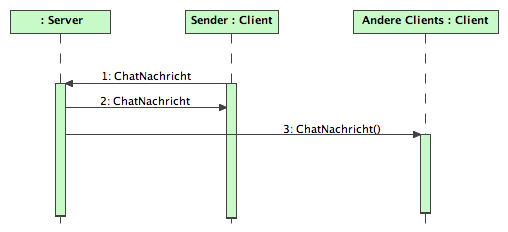
\includegraphics[width=\textwidth]{dienste_chat}
	\caption{Sequenzdiagramm Chat}
	\label{fig:dienste_chat}
\end{figure}

\clearpage
\section{Externes Design}

Das externe Design zeigt einen Entwurf für die Fenster des Spiels, wie sie ungefähr implementiert werden.

\subsection{Verbinden}

Beim Starten des Spiels wird der Spieler aufgefordert, die Serverdaten zur Verbindung und seinen Spielernamen einzugeben.

\begin{figure}[h]
	\centering
	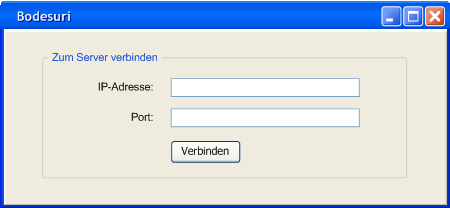
\includegraphics[width=0.7 \textwidth]{gui_verbindung}
	\caption{Design Verbinden}
	\label{fig:gui_verbindung}
\end{figure}

\clearpage

\subsection{Lobby}
\label{externes_design_lobby}

In der Lobby können die Spieler einen Partner für das Spiel auswählen\footnote{Wurde nicht implementiert.}. Der ausgewählte Partner muss die Anfrage akzeptieren, um die Gruppe zu bilden. Sobald der Spieler bereit ist, das Spiel zu beginnen, wählt er im Spielstatus "<bereit"> aus. In der Zwischenzeit können sich die Spieler im Chat unterhalten.

\begin{figure}[h]
	\centering
	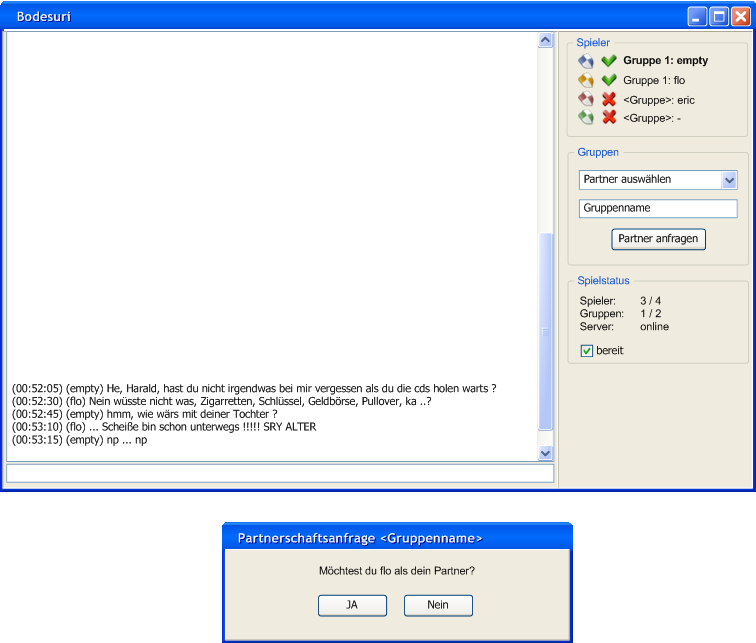
\includegraphics[width=0.9 \textwidth]{gui_lobby}
	\caption{Design Lobby}
	\label{fig:gui_lobby}
\end{figure}

\clearpage

\subsection{Spiel}
\label{externes_design_spielbrett}

Das Spiel besteht aus verschiedenen Views:
\begin{itemize}
	\item In der BrettView wird das Spielbrett mit den Feldern und Spielfiguren dargestellt.
	\item In der SpielerView werden die einzelnen Spieler mit Gruppenzugehörigkeit aufgelistet.
	\item Die KartenView beinhaltet die Karten des Spielers.
	\item In der ChatView können sich die Spieler unterhalten.
\end{itemize}

\begin{figure}[h]
	\centering
	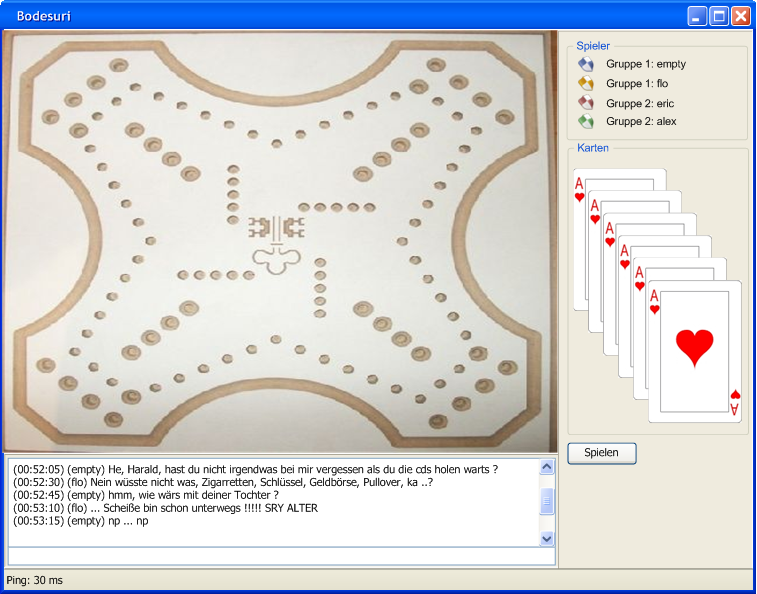
\includegraphics[width=0.9 \textwidth]{gui_spiel}
	\caption{Design Spiel}
	\label{fig:gui_spiel}
\end{figure}

\clearpage
\section{Designentscheidungen}

Im Verlauf des Projekts mussten wir einige Entscheidungen zum Design treffen. In den nachfolgenden Abschnitten wird der Hintergrund dazu erklärt und mit der Erwägung verschiedener Lösungsansätze auf die schliesslich implementierte Lösung hingearbeitet.

\subsection{Zustandsautomat}
Unser Spiel hat einen komplexen Ablauf, sowohl auf der Client- als auch auf der Serverseite. Der grösste Teil der Abläufe wird von Events im UI oder von Netzwerk-Nachrichten ausgelöst. Darum haben wir uns entschlossen, den Spielablauf in einem Zustandsautomaten zu verpacken.

Damit ist es möglich, den Programmablauf, der sonst in komplexem nacheinander aufzurufendem Programmcode verpackt wäre, in verschiedene Klassen auszulagern und den \emph{Gap} zwischen dem Code und den in der Elaboration gezeichneten Zustandsdiagrammen klein zu halten.

\subsection{Synchronisation UI/Automat}

Bodesuri verwendet für die Ablaufsteuerung und die interne Zustandssynchronisation zwischen Client und Server Zustandsautomaten. Der Zustandsautomat des Clients ist zusätzlich noch für die saubere Einbindung der darüber liegenden Schicht verantwortlich, zurzeit das GUI mit seinem Controller. Es stellte sich früh heraus, dass auch GUI und Automat gut synchronisiert werden müssen, so muss z.\,B. die Kartenauswahl im GUI deaktiviert werden, sobald eine Karte gewählt wurde. Wird dies nicht gemacht, kann der Automat bei Fehleingaben (der Benutzer wählt eine weitere Karte obwohl bereits getauscht) Events erhalten, welche in einem anderen Zustand gar keinen Sinn mehr ergeben und zu einer Exception führen.

Die offensichtliche Lösung für das Problem wäre eine kontrollierte Aktivierung und Deaktivierung aller GUI-Elemente in den betroffenen Zuständen, sprich das GUI in den Zustandsablauf einzubinden. Zum Beispiel könnte der Zustand Kartenwahl bei Zustandseintritt die Auswahl aktivieren und beim Verlassen des Zustands wieder deaktivieren. Eine solche Lösung ist aber leider auch mit Problemen verbunden. Das GUI und seine Komponenten laufen in eigenen Threads und können noch während der Verarbeitung des Zustands weiter agieren. Zum Beispiel könnte sich der Automat in der Verarbeitung der Kartenwahl befinden während das GUI, im Glauben es sei immer noch im gleichen Zustand, einen weiteren Kartenwahl-Event auslösen. Passiert dies, führt es höchstwahrscheinlich zu einem unerwarteten Event (Out-Of-State-Event) und somit zum kontrollierten, aber sinnlosen, Absturz.

Damit diese offensichtliche Lösung (zustandsbewusstes GUI) funktionieren könnte, müsste die Event-Verarbeitung von GUI und Automaten irgendwie koordiniert werden.

Folgende Varianten standen zur Auswahl:

\begin{itemize}
	\item GUI-Elemente werden bereits im ActionHandler des GUIs deaktiviert
	\begin{itemize}
		\item \textbf{Vorteil:} Keine Race-Conditions möglich
		\item \textbf{Nachteil:} Viel Zustandslogik im GUI, Erweiterungen sind aufwändig ("<in welchen Handlers muss ich das noch deaktivieren">)
	\end{itemize}
	\item GUI blockiert bis Automat abgearbeitet wird / Synchrone Event-Verarbeitung
	\begin{itemize}
		\item \textbf{Vorteil:} Keine Race-Conditions möglich, einfache Handhabung seitens GUI
		\item \textbf{Nachteil:} GUI könnte unter Umständen träge wirken, komplizierte Umsetzung
	\end{itemize}
\end{itemize}

Ein ganz anderer Ansatz besteht darin, das GUI ganz von den Zuständen zu entkoppeln. Das GUI könnte jederzeit Events auslösen und es wäre die Aufgabe des Zustandsautomaten zu erkennen, ob diese Events im gegebenen Zustand Sinn ergeben oder halt eben nicht. Natürlich könnten einzelne Bedienelemente trotzdem Zustandsabhängig aktiviert \& deaktiviert werden (z.\,B. um die Benutzerfreundlichkeit zu erhöhen) aber die korrekte Funktion des Automaten wäre davon unabhängig, er könnte problemlos mit "<Out-Of-State-Events"> umgehen.

\textbf{Vorteile:}
\begin{itemize}
	\item GUI simpler, entkoppelt von Zuständen
	\item Keine komplizierte Synchronisation mit Swing
\end{itemize}

\textbf{Nachteile:}
\begin{itemize}
	\item Automat ist bei GUI-Events weniger strikt\footnote{Der Automat ist in allen anderen Bereichen sehr strikt, was eine frühe Fehlererkennung mit sich bringt. Zum Beispiel können bei Events zur Synchronisation mit dem Server keine \emph{Fehler} toleriert werden.}
\end{itemize}

Wir entschieden uns aufgrund der genannten Vorteile für die Implementierung der dritten Variante.

\subsection{Kommunikation GUI/Automat}

Im Laufe der Phase \emph{Construction 1} zeigten sich erste Schwierigkeiten mit der Implementierung des Controllers. Ursprünglich war geplant, dass sich alle UI-Elemente, die direkt durch den Automaten kontrolliert werden müssen, beim Controller registrieren. Der Controller hätte dann die Elemente, je nach Anweisung des Automaten, direkt manipulieren können. Leider hatte dies verschiedene Nachteile. Einerseits war mit diesem System das GUI und der Controller extrem eng verknüpft. Dies zeigte sich in verschiedensten zyklischen Abhängigkeiten. Andererseits war aber auch der Code teilweise schwer nachvollziehbar, weil plötzlich gewisse GUI-Logik in Mouse-Adaptern und ähnlichen Klassen steckte. Zusätzlich wurde, da jede auch noch so kleine UI-relevante Zustandsänderung gemeldet werden musste, der Controller immer komplizierter und war schwer zu durchschauen.

Wir analysierten die Situation und kamen nach einigen Diskussionen zum Schluss, dass ein alternatives Kommunikations-Modell die Kommunikation vereinfachen könnte. Zusätzlich setzten wir uns das Ziel, dass das GUI nichts mehr direkt über den GUIController wissen muss. 

Das neue Modell sah vor, dass der grosse Teil der Kommunikation über Observer passieren sollte. Also z.\,B. das Feld weiss von sich selber ob es zurzeit ausgewählt ist und meldet etwaige Zustandswechsel über Observer-Event an das GUI. Dieses neue Konzept stellte uns plötzlich vor ein weiteres Problem. Wir sahen, dass wir plötzlich ganz viele, für die PD nicht relevante, Informationen in der Problem-Domain hätten ablegen müssen. Auf Grund der komplexen Regel-Logik war die Problem-Domain jedoch bereits relativ kompliziert. 

Um eine Vergrösserung der Problem-Domain zu verhindern begannen wir, einige ihrer Teile in Form von \emph{Dekoratoren} in der Applikationsschicht abzubilden. Diese Dekoratoren bildeten mehr oder minder dieselbe Funktionalität\footnote{Dafür leiteten sie die Methodenaufrufe einfach direkt in die darunterliegende Schicht weiter.} ab und observierten die jeweils dekorierten Objekte in der Problem-Domain. Zusätzlich beinhalteten sie aber Felder und Logik, die nur für die Applikationschicht relevant sind, so zum Beispiel den aktuellen Selektierungszustand.

Mit diesem System wird das UI über alle Änderungen informiert, sei es nun eine Änderung am PD-Objekt oder am Dekorator in der Applikationsschicht. Sollte eine alternative GUI-Implementierung kein Interesse an diesen Events haben, kann es diese entweder ignorieren oder sich gar nicht erst als Observer registrieren.

Diese Änderungen zog grössere Arbeiten nach sich, aber unter dem Strich hat sie die Logik bedeutend einfacher gemacht. Es hätte jedoch einige doppelte Arbeit erspart werden können, wenn diese bessere Lösung früher erkannt worden wäre.

Der Kontroller erstreckt sich nun über folgende Klassen. Diese Verteilung wurde so gewählt, um alle zyklischen Abhängigkeiten zu eliminieren. Damit ist es nun möglich, völlig unabhängige Kontroller zu implementieren.
\begin{enumerate}
	\item Interface applikation.client.controller.Steuerung.
	\item Abstrakte Klasse applikation.client.controller.Controller.
	\item Implementierende Klassen ui.GUIController und applikation.bot.BotController.
\end{enumerate}

\subsection{Multitier-Architektur des Servers}
Der Server wurde in mehrere Schichten und vertikal angeordnete Partitions aufgeteilt. Diese Hierarchie hat sich deshalb als erforderlich erwiesen, da sonst Abhängigkeiten von tieferliegenden zu höherliegenden Schichten entstehen würden.

\subsection{Applikationsschicht}
Die Applikationsschicht wurde eingeführt, weil es wegen der Netzwerkfähigkeit viel Synchronisationsarbeit (z.\,B. für Zustände) gibt. Sie hat folgende Hauptaufgaben:
	\begin{itemize}
		\item Zustandssynchronisation als erste Vorstufe der Netzwerkkommunikation. Spezifische Nachrichten werden eingepackt, an die darunterliegenden Schichten weitergeleitet, um dann über das Netzwerk verteilt und empfangen zu werden.
		\item Controller-Komponente des MVC-Konzeptes, welche die Ereignisse im UI abfängt und verarbeitet, sowie Änderungen in der Problem-Domain an das UI weiterleitet.
	\end{itemize}

\subsection{Regelverstoss als Exception}

Wenn eine Zug getätigt werden soll, wird zuerst mit den Angaben des Benutzers eine ZugEingabe zusammengestellt. Diese wird dann vom Regelsystem auf Gültigkeit geprüft (Methode \texttt{validieren}), wobei es zwei mögliche Ergebnisse gibt:
\begin{itemize}
	\item Die ZugEingabe ist gültig und das Resultat ist ein ausführbarer Zug, der von der Regel zusammengestellt wurde.
	\item Die ZugEingabe ist ungültig und das Resultat ist ein Verstoss mit einer Erklärung, warum die ZugEingabe ungültig ist.
\end{itemize}

Eine Möglichkeit, diese beiden Ergebnisse von einer Methode zurückzugeben ist, eine Klasse zu machen, die beides beinhalten kann, oder eine Basisklasse mit zwei sehr unterschiedlichen Resultat-Unterklassen. Mit dieser Variante wird jedoch sowohl der Code der \texttt{validieren}-Methode als auch der aufrufende Code komplizierter als nötig, da immer eine Fallunterscheidung gemacht werden muss. Wird zum Beispiel der Code von \texttt{validieren} in mehrere kleine Untermethoden zerlegt, muss bei jedem Aufruf der Rückgabewert geprüft werden und je nachdem mit der Validierung weitergemacht oder aufgehört werden.

Eine zweite Variante wäre, das Ergebnis der letzten Validierung in einer ständig vorhandenen Klasse zu speichern, wo es bei Bedarf abgerufen werden kann. Der Nachteil daran ist, dass das Ergebniss entkoppelt vom Aufruf von \texttt{validieren} an einem anderen Ort abgeholt werden muss, was nicht intuitiv ist und die beiden Klassen sehr stark voneinander Abhängig macht.

Die dritte und schliesslich implementierte Variante ist, bei Gültigkeit einen Zug zurückzugeben und andernfalls eine Exception des Typs \texttt{RegelVerstoss} zu werfen. Damit sind die Nachteile beider oben genannten Varianten beseitigt, die beiden verschiedenen Resultate sind sauber getrennt und aufrufender Code wird zudem noch gezwungen, den Fehlerfall zu behandeln (\texttt{RegelVerstoss} ist \emph{checked}).

\subsection{Mögliche Züge in Regel}
\label{sub:moegliche_zuege_in_regel}

Die folgenden beiden Methoden in \texttt{Regel} haben ganz ähnliche Funktionen:

\begin{itemize}
	\item \texttt{istZugMoeglich} findet heraus, ob mit dieser Regel für den übergebenen Spieler noch ein Zug möglich ist.
	\item \texttt{getMoeglicheZuege} findet alle möglichen ZugEingaben mit dieser Regel für den übergebenen Spieler.
\end{itemize}

Wie werden diese implementiert? Es wäre natürlich möglich, \texttt{istZugMoeglich} anhand von \texttt{getMoeglicheZuege} zu definieren, indem geschaut wird, ob diese eine leere Liste zurückgibt. Dies kann aber rechenintensiv sein, da in jedem Fall alle Möglichkeiten durchgegangen werden, obwohl das nicht nötig ist.

Eine andere Variante wäre, den Code einfach zu kopieren und jeweils einen kleinen Teil darin anzupassen, um den Anforderungen an die beiden Methoden gerecht zu werden. Dies hätte aber duplizierten Code zur Folge und eine erschwerte Anpassbarkeit, da jeweils in zwei Funktionen der gleiche Code angepasst werden müsste.

Deshalb entschieden wir uns, die folgende Variante zu implementieren. Es wird eine interne (\emph{protected}) dritte Methode erstellt, die \texttt{liefereZugEingaben} heisst. Diese übernimmt die gleichen Argumente wie die beiden obengenannten Methoden und zusätzlich noch ein Objekt des neuen Typs \texttt{ZugEingabeAbnehmer}. Die Methode liefert dem Abnehmer über \texttt{nehmeEntgegen} eine Zugeingabe und stellt anhand des Rückgabewertes fest, ob mit der Suche abgebrochen werden soll.

Die Methode \texttt{istZugMoeglich} ruft \texttt{liefereZugEingaben} mit einem Abnehmer auf, der nur auf die erste Zugeingabe wartet, einen Wert setzt, und signalisiert, dass abgebrochen werden kann. Danach wird der Wert ausgelesen und je nachdem zurückgegeben, ob ein Zug möglich ist oder nicht.

Für \texttt{getMoeglicheZuege} wird ein Abnehmer verwendet, der alle Zugeingaben speichert und immer zurückgibt, dass er weitere wünscht.

Mit dieser Lösung ist der Code zur Findung von Zugeingaben nur einmal vorhanden und die beiden Methoden laufen trotzdem nur so lange wie nötig.

\subsection{Siebnerzug}

Da die Karte Sieben beliebig auf die eigenen Figuren aufgeteilt werden kann, befürchteten wir zu Beginn, dass es sich bei der Erfassung eines Zuges mit der Sieben um eine schwierige Angelegenheit handelt. Ein Beispiel für ein Problem beim Erfassen eines solchen Zuges ist, dass unter Umständen eine Figur nach Hause geschickt werden muss, damit sie für weitere Teilzüge nicht mehr zur Verfügung steht. Dazu müsste der erfasste Teilzug bereits validiert werden, was das Zurücknehmen von bereits erfassten Teilzügen und somit das Abbrechen eines Siebnerzuges verunmöglicht. Eine mögliche Lösung wäre, beim Beginn eines Siebnerzuges, das ganze Brett zu klonen und bei einem Abbruch wieder zurück zu holen. Da verschiedene Observer, welche Teile des Brettes überwachen, umgeleitet werden müssten, ist diese Lösung zu komplex.

Es bot sich aber eine viel einfachere und beinahe gleich flexible Lösung an. Ein Siebnerzug wird erst validiert, wenn insgesamt Sieben Felder gefahren wurden. Um die erfassten Teilzüge trotzdem visualisieren zu können, werden beim Ziel jedes Teilzuges halbtransparente Spielfiguren (wir nennen sie "<Geister">) platziert. Damit kann der Spieler sehen, dass sein Zug erfasst aber noch nicht komplett ist. Theoretisch ist es damit zwar möglich mit einer Figur, die nicht mehr auf dem Feld sein sollte, zu Fahren, dieser Fehler wird vom Regelsystem bei der Validierung aber erkannt und mit einer Fehlermeldung gemeldet.

\clearpage
\section{Eingetretene Risiken}
\label{eingetretene_risiken}

Im Projektplan hatten wir zu Beginn des Projekts einige Risiken aufgezählt, die während des Projekts eintreten könnten. Die folgenden Risiken aus dem Bereich "<Probleme mit Technologien"> sind tatsächlich eingetreten und werden nachfolgend erklärt.

\subsection{RMI}
\label{sub:rmi}

Im Verlauf der ersten Tests mit RMI stellte sich schnell heraus, dass RMI weit mehr kann als für das Projekt notwendig wäre und es dem Projekt somit unnötig Komplexität hinzufügt. Andererseits stellt RMI  einige Anforderungen an die Client/Server-Struktur, die sich nur schwer mit den Projektanforderungen decken lassen. So kann RMI nur erschwert hinter Firewalls betrieben werden und eine Kommunikation über ein durch NAT\footnote{Network Adress Translation. Firewall-Feature welches Netzbereiche auf andere Netzbereiche abbildet. Wird häufig verwendet, um private Adressbereiche im Internet hinter einer einzelnen Adresse zu verstecken.} verstecktes Netzwerk ist gar nicht erst möglich. Da die Internet-Zugangslösungen in den meisten Haushalten auf Firewalls und NAT basieren, könnte das Spiel von einem grösseren Teil der potenziellen Kundschaft gar nicht gespielt werden.

Wir entschieden uns aufgrund dieser Probleme, auf eine eigene Lösung umzusteigen, welche auf den Java-Klassen Socket und Object(Input|Output)Stream basiert. Insgesamt gingen etwa 10 Stunden Arbeit für diese Umstellung verloren.

\subsection{Java 2D}
\label{java_2d}

Nachdem das CLI (Command Line Interface) erstellt war, entwarfen wir ein GUI dafür, das die Felder und Figuren darstellen sollte. Mit Java 2D ist das Zeichnen sehr einfach, da man die Koordinaten der zu zeichnenden Elemente angeben kann. Doch mussten wir leider feststellen, dass das Ansprechen eines Objektes etwas komplizierter ist. So muss zum Beispiel bei einem Mausklick das geklickte Objekt über die Koordinaten ermittelt werden. Ausserdem muss man sich um das Aktualisieren der Anzeige bei Veränderungen selber kümmern.

In einem zweiten Versuch erstellten wir das selbe Spielbrett mit Swing und wir kamen zum Schluss, dass dies die einfachere Methode ist. Die Objekte können mit einem speziellen Layout auch auf Koordinaten genau platziert werden und Klicke darauf kann man wie gewohnt mit einem MouseListener abfangen. Als Objekt kann man zum Beispiel ein Label mit einem Icon verwenden. Dies reicht für ein Brettspiel vollkommen aus.

Aus diesen Gründen haben wir uns dazu entschlossen, für das GUI als einzige Technologie Swing einzusetzen. Insgesamt gingen 7.5 Stunden Arbeit für diese Umstellung verloren.

\clearpage
\section{Besser als erwartet}

Einige Dinge, von denen wir dachten, sie würden viel Zeit brauchen, die aber einfacher zu implementieren waren als erwartet.

\subsection{Serialisierung}

Um Objekte über das Netzwerk zu schicken, müssen sie serialisiert werden, das heisst den Zustand eines Objektes so in eine binäre Form zu bringen, dass es an einem anderen Ort oder zu einem anderen Zeitpunkt eingelesen werden kann, um wieder den ursprüngliche Zustand des Objektes zu erhalten.

Normalerweise ist das Objekt an einem Ort vorhanden und am anderen nicht. In unserem Fall müssen aber alle Objekte der Problem-Domain sowohl auf jedem Client als auch auf dem Server bereits existieren. Wenn nun ein Objekt übertragen wird, wird am empfangenden Ort ein neues Objekt erstellt, das zwar die gleichen Daten hat, aber nicht die gleiche Identität (gleiche Speicheradresse) wie das bereits vorhandene Objekt. Wenn dann mit dem empfangenen Objekt etwas gemacht wird, wird das z.\,B. vom GUI, welches das bereits vorhandene Objekt observiert, nicht bemerkt.

Für diese Problemstellung wird also ein Mechanismus gebraucht, der bei der Deserialisierung nicht neue Objekte, sondern die bereits vorhandenen zurückliefert. Dies ist bei der Java-Serialisierung mit den beiden Methoden \texttt{writeReplace} (beim zu schreibenden Objekt) und \texttt{readResolve} (beim einzulesenden Objekt) möglich, wo jeweils Objekte zurückgegeben werden können, die dann anstelle der ursprünglichen verwendet werden.

Damit ist die Grundlage für eine Serialisierung wie wir sie brauchen vorhanden. Darauf aufbauend ist nun noch eine eindeutige Codierung der Objekte nötig, die auf jedem Rechner gleich sein muss. Der Ablauf einer Übertragung eines Objektes ist dann wie folgt:

\begin{enumerate}
	\item Beim zu schreibenden Objekt (zum Beispiel \texttt{Feld}) wird in \texttt{writeReplace} ein \texttt{CodiertesObjekt} zurückgeliefert, welches nur einen Code enthält, der dieses Objekt eindeutig identifiziert (zum Beispiel \texttt{Feld 47}).
	\item Das stellvertretende Objekt wird über das Netzwerk geschickt.
	\item Beim Einlesen von \texttt{CodiertesObjekt} wird von Java die Methode \texttt{readResolve} aufgerufen, welche in einer Tabelle zum Code das dazugehörige Objekt nachschaut und zurückgibt.
\end{enumerate}

Dank der Serialisierungsschnittstelle von Java ist diese Lösung transparent. Der Vorgang ist in Abbildung~\vref{fig:dienste_serialisierung} detailliert als Sequenzdiagramm dargestellt.

\subsection{Steuerung der Partnerfiguren}

Wenn ein Spieler mit all seinen Figuren in den Himmel ziehen konnte, wird im Spiel der Endmodus aktiviert, in welchem es dem fertigen Spieler ermöglicht wird, mit den Figuren seines Partners zu ziehen.

Zu Beginn gingen wir von der Annahme aus, dass man dieses Verhalten im Regel- und Zugssystem als separat zu behandelnden Spezialfall implementieren muss. Bei der Umsetzung hat sich dann jedoch gezeigt, dass ein Spieler einfach in die Rolle des Partners schlüpfen kann und so das vorhandene Regel- und Zugsystem genau gleich auf diese Zugeingaben reagiert.

Ein wichtiger Bestandteil der Lösung ist es, die Partnerschaften, welche auf dem Server gebildet werden, konsistent auf die Clients zu synchronisieren. Dies ist darum sehr wichtig, da beide Teile -- der Client und der Server -- die Zugeingaben validieren und es darum ansonsten entweder auf einem Client oder dem Server zu einem Regelverstoss (fehlgeschlagene Validierung) führen würde. Bei der Validierung eines Zuges wird nun zuerst der betroffene Spieler ermittelt. Dies ist immer der Spieler, für den der Zug ausgeführt wird oder anders ausgedrückt der Spieler, dem die Figur gehört. Im Normalfall ist dies der Spieler selbst. Ist der Spieler jedoch fertig, so wird der Zug automatisch für seinen Partner ausgeführt.

\subsection{Handhabung des Jokers in Bot und Server}

Wenn man die Joker-Karte spielt, kann man auswählen, als welche andere Karte man sie einsetzen möchte. Darum ist die Regel des Jokers eine RegelVeroderung aller Regeln der anderen Karten.

Für den Bot müssen alle Züge gefunden werden, die mit einer Karte möglich sind. Um den Joker einsetzen zu können, muss keine Spezialbehandlung gemacht werden, da die RegelVeroderung einfach alle möglichen Züge der enthaltenen Regeln sammelt und zurückgibt.

Auch auf dem Server ist der Joker kein Spezialfall. Er erhält vom Client eine ZugEingabe mit dem Joker als Karte und einer Bewegung (oder einer Liste von Bewegungen im Falle der Sieben). Daraufhin validiert er die ZugEingabe, was einen Aufruf von \texttt{validieren} der RegelVeroderung zur Folge hat. Diese ist gültig, sobald eine ihrer enthaltenen Regeln gültig ist. Nach der Validierung trägt der Server die Joker-Karte aus den Karten des Spielers aus.

\subsection{Bot}

Als das erste Mal die Idee auftauchte, einen zu Bot implementieren, schien dies ein Ding der Unmöglichkeit zu sein. Im Laufe der Weiterentwicklungen der Problem-Domain entdeckten wir aber eine Funktionalität, die wir auch für den Bot relativ gut brauchen konnten. Und zwar schreiben die Dog-Regeln vor, dass die aktuelle Runde nur aufgegeben werden darf wenn kein Zug mehr möglich ist. Also selbst wenn nur noch für den Spieler \emph{negative} Züge möglich sind, muss er die Züge ausführen. Hierfür muss die PD herausfinden, ob und welche Züge noch möglich sind.

Dieselbe Logik konnte nun auch für den Bot verwendet werden. Anstatt den erstbesten möglichen Zug zu suchen muss sie alle möglichen Züge zusammensammeln und anschliessend dem Bot zur Auswahl stellen. Wie diese beiden ähnlichen Methoden implementiert wurden, kann im Abschnitt~\vref{sub:moegliche_zuege_in_regel} nachgelesen werden.

Der aktuelle Bot (Klasse StupidBot) wählt von diesen Zügen zufällig irgendeinen Zug aus und verwendet ansonsten keine weitere Logik. Interessanterweise wird aber eine Partie mit vier solchen Bots trotzdem innerhalb brauchbarer Zeit (ca. 900 Züge) durchgespielt. Gegen einen Menschen haben sie natürlich keine Chance, aber sie erwiesen sich in zwei Situationen als erstaunlich nützlich:

\begin{itemize}
	\item \textbf{BodesuriDemo:} Die main-Methode der Klasse BodesuriDemo startet einen Server, drei Bots und einen normalen Client. Die Demo ist ein einfacher und bequemer Weg um das Spiel auszuprobieren. Für reine Demo-Zwecke genügt der Bot vollkommen.
	\item \textbf{ServerTest:} Eine Bot-Partie ohne GUI dauert ungefähr 20 Sekunden und eignet sich überraschenderweise erstaunlich gut um grosse Teile der Codebasis zu testen. Der Test ist relativ simpel, er ist nur erfolgreich wenn sich das Spiel in brauchbarer Zeit erfolgreich beendet. Da die ganze Client/Server Logik relativ strikt ist, führt ein kleiner Fehler in der Regel sofort zu einem Absturz und somit zu einem Fehlschlagen des Tests.
\end{itemize}

\clearpage
\section*{Glossar}
\begin{itemize}
	\item \textbf{Veroderung}: Das logische Oder von Dingen. In unserem Fall Regeln.
	\item \textbf{Spielers}: Wurde im Quellcode verwendet um klar auszudrücken, dass es sich um mehrere Spieler (z.B. ein Array) handelt.
	\item \textbf{Konkrete Karte}: Die Karte, für die ein Joker steht.
	\item \textbf{Aktiver Zustand}: Ein Zustand der auf einen Event wartet um in den nächsten Zustand über zu gehen.
	\item \textbf{Passiver Zustand}: Ein Zustand der direkt in den nächsten Zustand über geht. Quasi ein Epsilon-Übergang.
\end{itemize}

\clearpage
\listoffigures

\end{document}
